\chapter{Разработка систем компьютерного зрения на основе глубоких нейронных сетей}

Научные и практические результаты, полученные в рамках данной диссертационной работы, внедрены и используются на следующих предприятиях Республики Беларусь:

\begin{easylist}
	& <<Intelligent Semantic Systems>> (г. Минск) при разработке подсистемы компьютерного зрения для осуществления распознавания объектов;
	& ОАО <<Савушкин продукт>> (г. Брест) при разработке системы автоматического контроля качества нанесения маркировки продукции;
	& в учебном процессе учреждения образования <<Брестский государственный технический университет>>.
 \end{easylist}

Сведения об использовании результатов диссертационной работы отражены в соответствующих актах внедрения, приведенных в приложении \ref{app:b}.

\section{Обнаружение солнечных панелей на аэрофотоснимках}

\subsection{Постановка задачи и обзор существующих решений}
По причине увеличивающейся доли использования солнечной энергии, спрос на фотоэлектрические элементы в мире постоянно растет. С начала 2010-х годов индустрия производства и поддержки солнечных панелей переживает стремительный рост. Так, по состоянию на 2022 год только в США в данной отрасли работает более 10000 компаний и 263.000 сотрудников \cite{seia}.

В связи с растущей популярностью этой технологии проблемы, связанные с обслуживанием солнечных панелей, также становятся актуальными. Многие сервисные компании заинтересованы в получении информации о потенциальных клиентах. Таким образом, анализ фотоснимков с целью обнаружения солнечных панелей и накопления статистической информации является актуальной задачей.

%Развитие теории обучения глубоких нейронных сетей [4] дало мощный импульс для разработки различных вариантов сверточных нейронных сетей, применяемых для решения задач распознавания и классификации. Появление технологии параллелизации вычислений с использованием GPU в свою очередь сделало такое обучение осуществимым за приемлемый отрезок времени.

Поставленная задача заключалась в разработке системы обнаружения солнечных панелей на изображениях с их последующей локализацией.

В статье Дж. Малофа \cite{malof2015} был описан подход, базирующийся на использовании SVM для автоматического обнаружения солнечных панелей, используя фотографии высокого разрешения, полученные с помощью спутника. В этом подходе сначала применяется операция предварительного скрининга, которая идентифицирует регионы, которые затем обрабатываются с целью выделения признаков. В качестве выходной информации, получаемой с помощью данной модели, выступает список регионов и доверительные значения, показывающие, насколько вероятно наличие солнечной панели в заданной области. Общая эффективность подхода определения наличия панелей в \cite{malof2015} составляет порядка 94\%. Однако, нужно отметить, что данный метод дает лишь приблизительную информацию о местонахождении панели. Оценки точности локализации панелей в работе не приводится.

В \cite{malof2016} используется подход, базирующийся на применении деревьев решений. Достигнутый показатель локализации панелей составил 90\% в случае использования определенных параметров алгоритма, а сам метод состоит из четырех стадий. В работе в качестве обучающей выборки используется Aerial Imagery Dataset, включающий изображения разрешением до 5000 Х 5000 пикселей \cite{bradbury2016}.

\subsection{Предлагаемый подход}

Предложенный нейросетевой алгоритм для обнаружения солнечных панелей отличается тем, что в качестве базовой модели используется сверточная нейронная сеть, которая показывает лучшие результаты при решении задач классификации и детекции объектов на изображениях. Другое важное отличие заключается в использовании фотографий низкого разрешения для обучения нашей модели (например, фото из Google Maps, нередко неудовлетворительного качества, см. рис. \ref{fig:example_of_images}). 

\begin{figure}[ht]
	\centering
	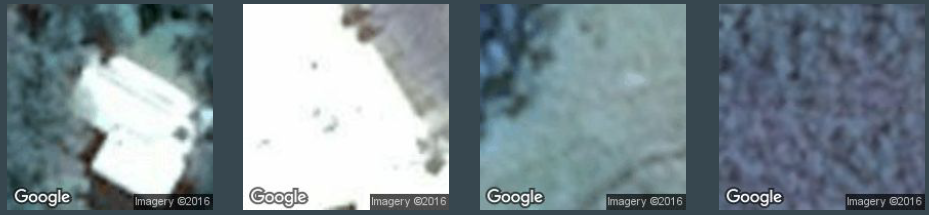
\includegraphics[width=16cm]{man-source/images/ch4/pic4-16.png}
	\caption{Примеры изображений низкого качества из обучающей выборки}
	\label{fig:example_of_images}
\end{figure}

Предлагаемая система обнаружения солнечных панелей включает два основных компонента, в составе которых используются предобученные глубокие нейронные сети (рис. \ref{fig:solar_system_arch}): 

\begin{easylistNum}
    & Классификатор для оценки наличия солнечной панели на аэрофотоснимке;
    & Детектор для локализации солнечной панели.
\end{easylistNum}

\begin{figure}[ht]
	\centering
	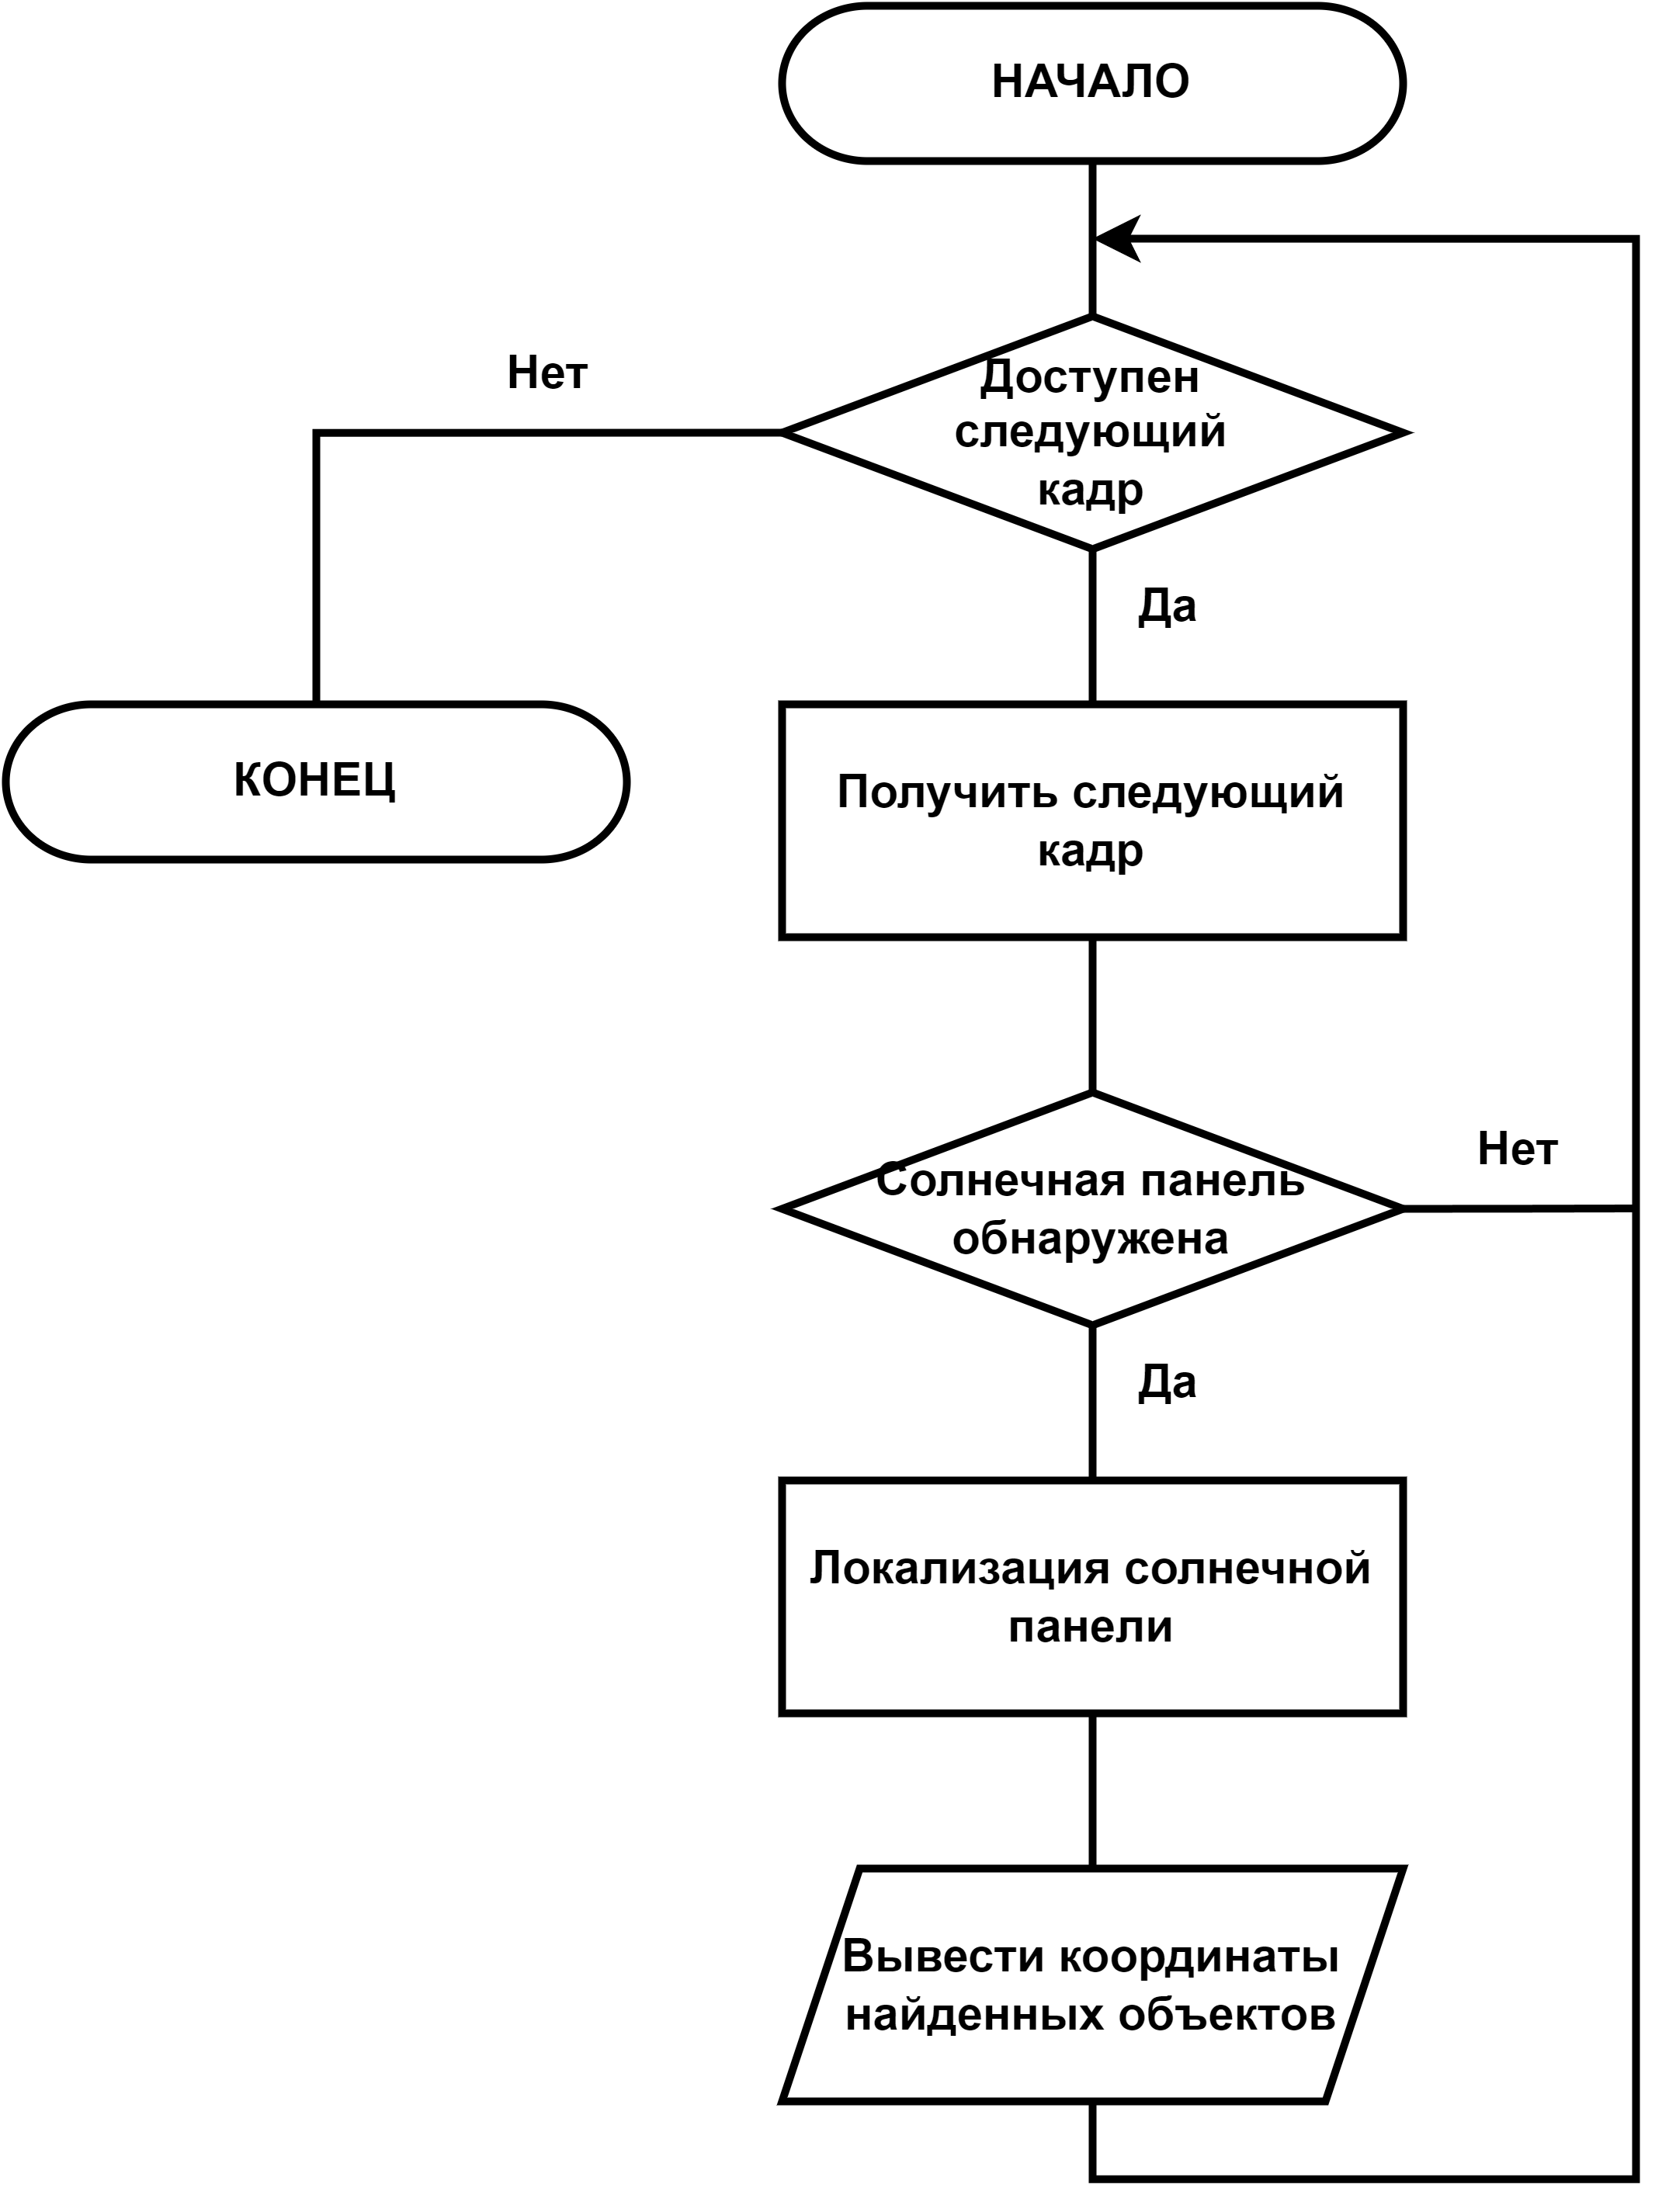
\includegraphics[width=12cm]{man-source/images/ch4/pic4-16a.png}
	\caption{Блок-схема работы системы обнаружения солнечных панелей}
	\label{fig:solar_system_arch}
\end{figure}

Двухэтапность в решении поставленной задачи позволяет существенно ускорить обработку изображений, большую часть которых занимают объекты, отличные от искомых (солнечных панелей), т.к. нейросетевые модели, используемые на этапе локализации, как правило, более ресурсоемки. Таким образом, модель первого этапа выполняет роль фильтра для последующей обработки. Тем самым предлагаемый алгоритм можно применять для последовательной обработки больших изображений.

\textbf{Классификатор для оценки наличия солнечной панели на аэрофотоснимке}. Для этой подзадачи применялся сверточный классификатор с архитектурой, представленной на рис. \ref{fig:used_cnn} [35]. 

Представленная нейронная сеть состоит из шести слоев. Первые три слоя являются сверточными и выполняют выделение высокоуровневых признаков. Последние три слоя представляют собой полносвязные слои нейронных элементов, решающие задачу классификации. Для всех слоев, кроме последнего, используется функция активации ReLU \ref{eq:relu_function}.

\begin{figure}[ht]
	\centering
	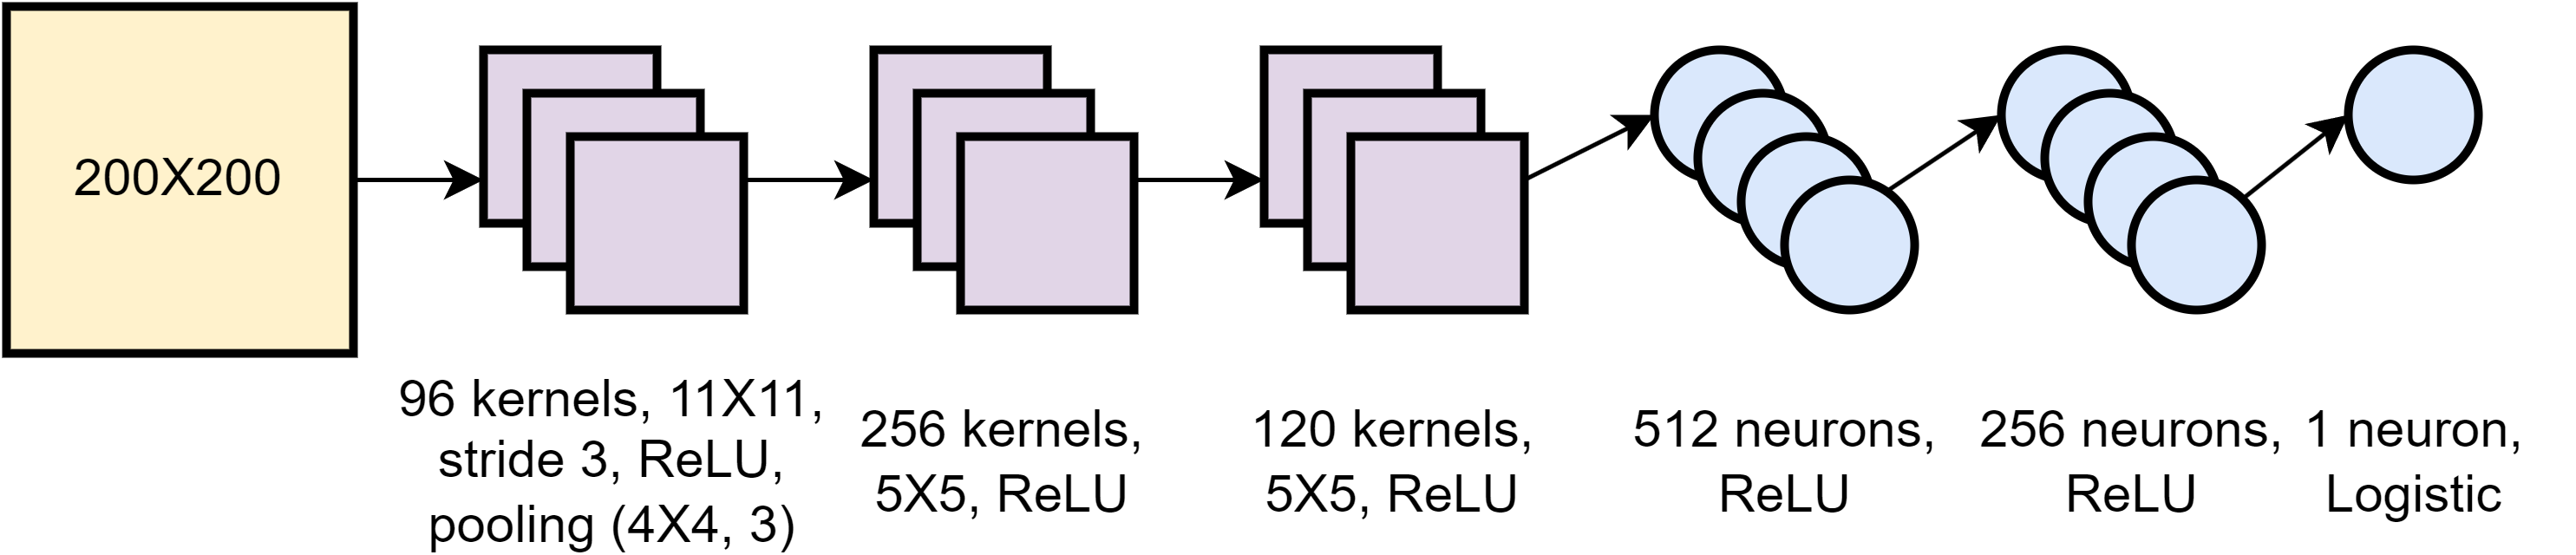
\includegraphics[width=17cm]{man-source/images/ch4/pic4-19.png}
	\caption{Архитектура используемой сверточной нейронной сети}
	\label{fig:used_cnn}
\end{figure}

\begin{equation}
    \label{eq:relu_function}
    ReLU(x) = max(0, x)
\end{equation}

В последнем полносвязном слое используется сигмоидная функция активации \ref{eq:sigmoid_function}.

\begin{equation}
    \label{eq:sigmoid_function}
    Logistic(x) = \frac{1}{1+e^{-x}}
\end{equation}

Дополнительно, на первом сверточном слое мы используем шаг, равный 3, с целью уменьшения размерности получаемых со сверточного слоя карт признаков.

Последний полносвязный слой модели содержит только один нейрон, по возвращаемому значению которого оценивается вероятность наличия солнечной панели на изображении. Для предобучения сверточной нейронной сети использовался предложенный метод REBA, метод стохастического градиентного спуска применялся на этапе <<тонкой настройки>>. 

\textbf{Детектор для локализации солнечной панели}. Для решения подзадачи локализации применялась глубокая нейронная сеть Faster-RCNN (Faster Region-based Convolutional Neural Network), базирующаяся на классификаторе ResNet-50 (\ref{fig:faster_rcnn}). Данная модель состоит из двух частей. Первая часть -- это классификатор ResNet-50, предобученный на выборке COCO \cite{lin2015}. Вторая часть -- это детектор, который представлен сверточной нейронной сетью, генерирующей координаты прямоугольных областей (боксов), содержащих в себе обнаруживаемые моделью объекты, и метки класса для каждой такой области с оценкой уверенности в данной метке (confidence score).

\begin{figure}[ht]
	\centering
	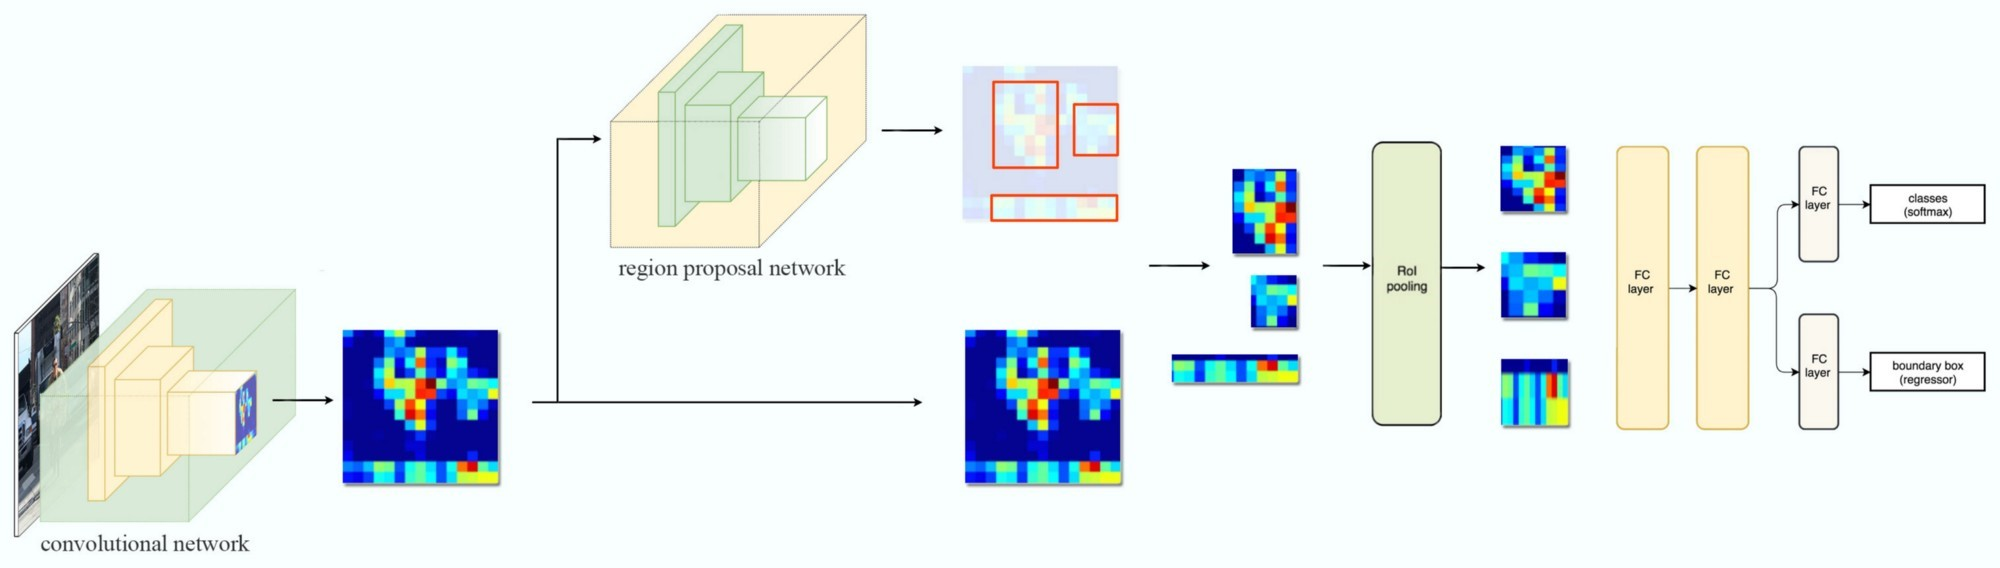
\includegraphics[width=17cm]{man-source/images/ch4/pic4-21.jpg}
	\caption{Глубокая сверточная сеть Faster-RCNN}
	\label{fig:faster_rcnn}
\end{figure}

Подобная архитектура модели обеспечивает получение высоких показателей эффективности при решении задач детекции объектов в системах, где общее время, затраченное на обработку и вывод результатов, некритично.

\subsection{Обучающая выборка}
В качестве исходных данных, используемых для формирования обучающей выборки для решения задачи обнаружения солнечных панелей, использовались цветные изображения Google Maps с разрешением 200 Х 200 пикселей (рис. \ref{fig:google_maps}).

\begin{figure}[ht]
	\centering
	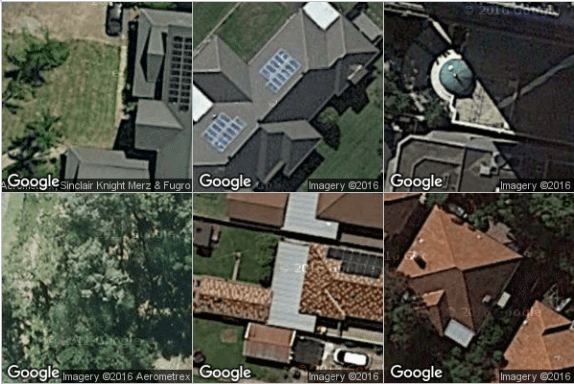
\includegraphics[width=12cm]{man-source/images/ch4/pic4-17.png}
	\caption{Примеры изображений из выборки Google Maps}
	\label{fig:google_maps}
\end{figure}

Для обучения модели классификатора использовалась выборка из 3347 фотографий (где 1643 изображения содержали солнечные панели, а 1704 -- не содержали), при этом 80\% исходной выборки формировали обучающую выборку, а 20\% - тестовую. Для обучения модели детектора использовалась выборка из 1000 изображений, 800 из которых было отнесено к обучающей, а 200 -- к тестовой выборкам.

Подготовка обучающей выборки для классификатора состояла в ручном переборе изображений и отнесении их к двум группам изображений -- содержащих солнечные панели и, соответственно, не содержащих. При подготовке обучающей выборки для детектора панелей также использовался ручной перебор изображений с определением для каждого характеристик прямоугольных областей, включающих солнечные панели (длина, ширина, координаты левого верхнего угла). При этом фиксировались все интересующие объекты (для случая множественных панелей). 

Выделение прямоугольных областей для некоторых изображений может не выглядеть целесообразным, например, случаи, когда панели расположены под углом к горизонтальной оси снимка и имеют вытянутую форму (рис. \ref{fig:background_dominate}). Однако, для таких фотографий удается получить приемлемые результаты локализации на тестовых данных, несмотря на то, что большая часть области включает фоновое изображение.
 
\begin{figure}[ht]
	\centering
	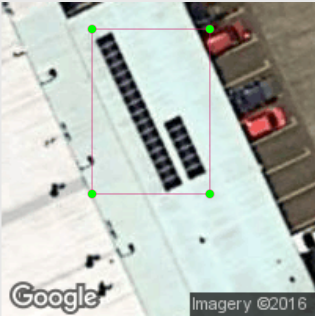
\includegraphics[width=8cm]{man-source/images/ch4/pic4-18.png}
	\caption{Пример изображения с преобладающим фоном}
	\label{fig:background_dominate}
\end{figure}

\subsection{Оценка качества обученных моделей}

Для оценки качества применялись две основные метрики. 

Первая метрика использовалась для оценки классификатора. В режиме тестирования модели применялось простое преобразование выходных данных -- пороговая функция вида:

\begin{equation*}
    b_s = I[y_s > 0,5]
\end{equation*}
где $y_s$ представляет реальное выходное значение CNN-сети, возвращаемое для $s$-го входного изображения выборки, $b_s$ -- бинаризованная форма, полученная вычислением индикаторной функции вида:

\begin{equation*}
    I[x] = 
    \begin{cases}
        1, & \text{x is True} \\
        0, & \text{x is False}
    \end{cases}
\end{equation*}

Метрика оценки рассчитывалась по формулам:

\begin{equation*}
    A = \frac{S}{L} * 100\%
\end{equation*}

\begin{equation*}
    S = \sum_{s=1}^L I[b_s = e_s]
\end{equation*}
где $e_s$ -- эталонное значение (метка), $L$ -- объем выборки. Таким образом, оценивается доля верных ответов, возвращаемых нейронной сетью.

Для оценки эффективности модели локализации использовалась метрика mAP.

Метрика mAP является стандартом де-факто метрик, используемых для оценки качества моделей, применяемых для детекции. Эта метрика используется вместе со своими модификацими, вычисленными для различных значений порога IoU. Так как для рассматриваемой задачи существует только один класс объектов, метрика mAP совпадает с AP.

Как известно, точность вычисляется по формуле:

\begin{equation*}
    P = \frac{TP}{TP + FP}
\end{equation*}
где \textit{TP} и \textit{FP} обозначают соответственно число истинно-положительных и ложно-положительных результатов детекции, и, соответственно, \textit{P} определяет долю корректных детекций в общем числе детекций, полученных моделью.

Значение \textit{TP} определяет общее количество прямоугольных областей, для которых величина \textit{IoU}, вычисленная относительно истинных областей (\textit{Ground-true box}), больше некоторого заданного порога (чаще всего выбирается порог 0,5). Таким образом, если величина \textit{IoU} для такой спрогнозированной области превысила 0,5, то детекция рассматривается как истинно-положительная. Если детекций для данной истинной области несколько, то выбирается одна детекция с самым большим значением \textit{IoU}, а остальные рассматриваются как \textit{FP}.

Усредненное значение по всем изображениям выборки дает величину AP:

\begin{equation*}
    AP = \frac{1}{L} \sum_{i=1}^L \frac{TP_i}{TP_i + FP_i}
\end{equation*}
где \textit{L} -- число изображений в выборке.

\subsection{Результаты обучения и тестирования}

Сверточная сеть для определения наличия солнечных панелей обучалась в течение 70 эпох, используя следующие параметры:

\begin{easylist}
    & скорость обучения -- 0,001;
    & моментный параметр -- 0,9;
    & weight-decay -- 0,0005;
    & размер мини-батча -- 20.
    & вероятность применения dropout для полносвязных слоев -- 0,5
\end{easylist}

Точность классификации для данной задачи, составила порядка \textbf{87,46\%} (см. таблица \ref{table:confusion_matrix}).

\begin{table} [H]
  \small
  \caption{Матрица ошибок}\label{table:confusion_matrix}
\begin{tabularx}{\hsize}{| X | X | X | X |}
  \hline
    & Спрогнозировано <<No>> & Спрогнозировано <<Yes>> & Точность,\% \\
    %\cline{2-3}
    \hline
    Ожидалось <<No>> & 325	& 32	& 91\\
    \hline
    Ожидалось <<Yes>>	& 52	& 261	& 83\\
    \hline
    Итого & 377	& 293	& 87\\
    \hline
\end{tabularx}
\end{table}

На рис. \ref{fig:roc_curve} изображена ROC-кривая, построенная для обученного классификатора.

\begin{figure}[ht]
	\centering
	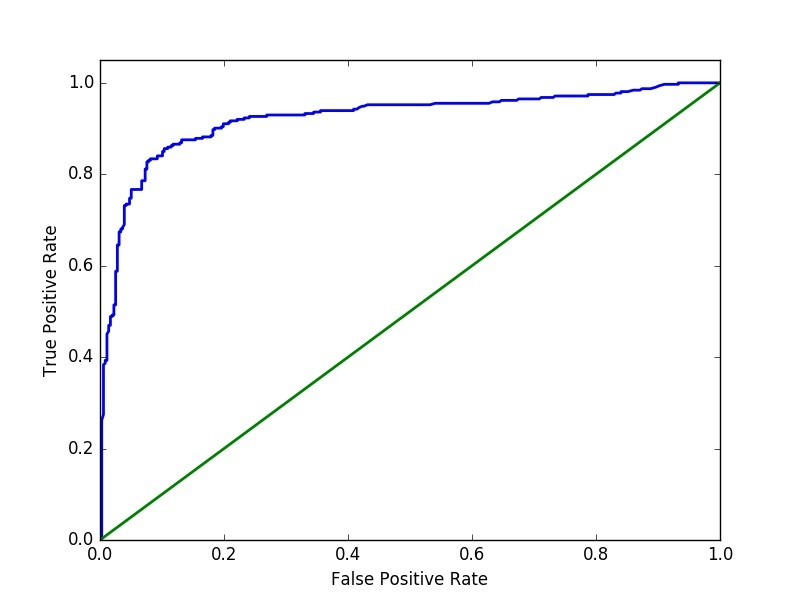
\includegraphics[width=11cm]{man-source/images/ch4/pic4-20.jpg}
	\caption{ROC-кривая для обученного бинарного классификатора, AUC = 0,92}
	\label{fig:roc_curve}
\end{figure}

Другие характеристики полученного классификатора: 
\begin{easylist}
    & полнота = 0,8339, 
    & специфичность = 0,9104, 
    & точность = 0,8907, 
    & F-мера = 0,8614.
\end{easylist}

Сеть для локализации объектов обучалась в течение 5000 итераций (под итерацией здесь понимается настройка параметров для одного случайного изображения из обучающей выборки), используя следующие параметры:

\begin{easylist}
    & скорость обучения -- 0,0003;
    & моментный параметр -- 0,9;
\end{easylist}

После выполнения обучения, проводилось исследование обобщающей способности сети с использованием тестовой выборки из 200 изображений. Полученный результат составил \textbf{\textit{AP}=0,9299}.

Визуализация выходов первого сверточного слоя, полученная после выполнения обучения, представлена на изображении \ref{fig:pic4-24}.

\begin{figure}[!ht]
	\centering
	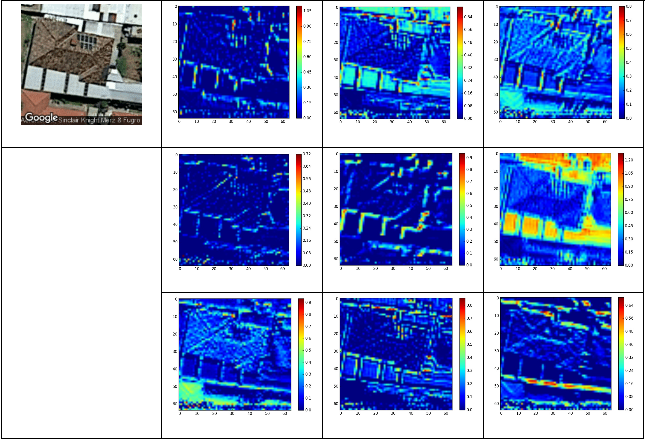
\includegraphics[width=16cm]{man-source/images/ch4/pic4-24.png}
	\caption{Визуализация выходов первого слоя НС}
	\label{fig:pic4-24}
\end{figure}

На рис. \ref{fig:test_results} изображены результаты детекции солнечных панелей на изображениях из тестовой выборки.

\begin{figure}[!ht]
	\centering
	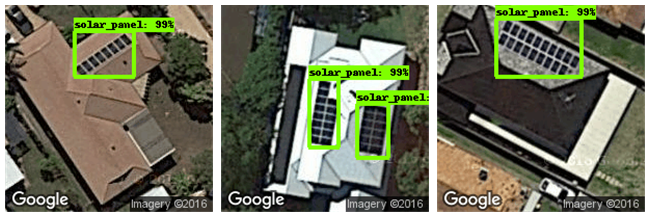
\includegraphics[width=16cm]{man-source/images/ch4/pic4-22.png}
	\caption{Результаты детекции для изображений из тестовой выборки}
	\label{fig:test_results}
\end{figure}

Как можно видеть, предложенный метод осуществляет достаточно точное обнаружение. На рис. \ref{fig:random_results} изображены результаты работы метода для произвольных изображений (не из тестовой выборки).

\begin{figure}[!ht]
	\centering
	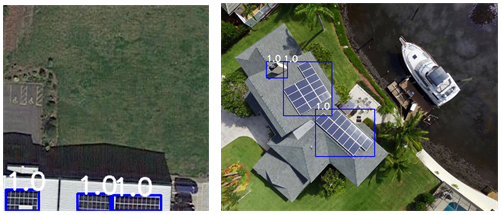
\includegraphics[width=16cm]{man-source/images/ch4/pic4-23.png}
	\caption{Результаты детекции для произвольных изображений}
	\label{fig:random_results}
\end{figure}

\section{Распознавание маркировки продукта}

\subsection{Постановка задачи и обзор существующих решений}

В основе конкурентности любого производства лежит выпуск разнообразной и качественной продукции. Качество является определяющим критерием при выборе клиентом того или иного продукта, а разнообразие позволяет охватить различные группы потенциальных покупателей. Системы, которые автоматизируют процесс проверки качества и при этом поддерживают многообразие продукции, выпускаемой на большом предприятии, имеют особую ценность. При этом процесс проверки качества осуществляется не только для самого продукта, но и для той упаковки и маркировки, которую видит покупатель. Так как упаковка формирует первоначальное впечатление о товаре, ее качество является одной из причин, которая дает покупателю основание для покупки. Маркировка как элемент упаковки, гарантирует покупателю сохранность продукции в течение указанного срока при соблюдении условий хранения.

В последнее время методы искусственного интеллекта в целом и машинного обучения в частности широко используются в промышленных системах, устанавливаемых на предприятиях для контроля за процессом производства. Интеллектуальные подсистемы позволяют упростить многие рутинные операции, проводимые для поддержания качества готовой продукции. Например, контроль за правильностью нанесения маркировки ранее производился исключительно оператором-человеком. Сейчас, с развитием теории компьютерного зрения, получившей значительный рывок благодаря постоянно развивающейся области обучения глубоких нейронных сетей, становится особенно актуальной разработка систем, позволяющих осуществлять рутинные операции быстрее и регулярнее, чем это мог бы сделать человек.

Поставленная задача заключалась в разработке системы распознавания маркировки продукции, производимой ОАО <<Савушкин продукт>>. Пример продукта с маркировкой, распознавание которой выполняется, представлен на рис. \ref{fig:digital_code}.

\begin{figure}[ht]
	\centering
	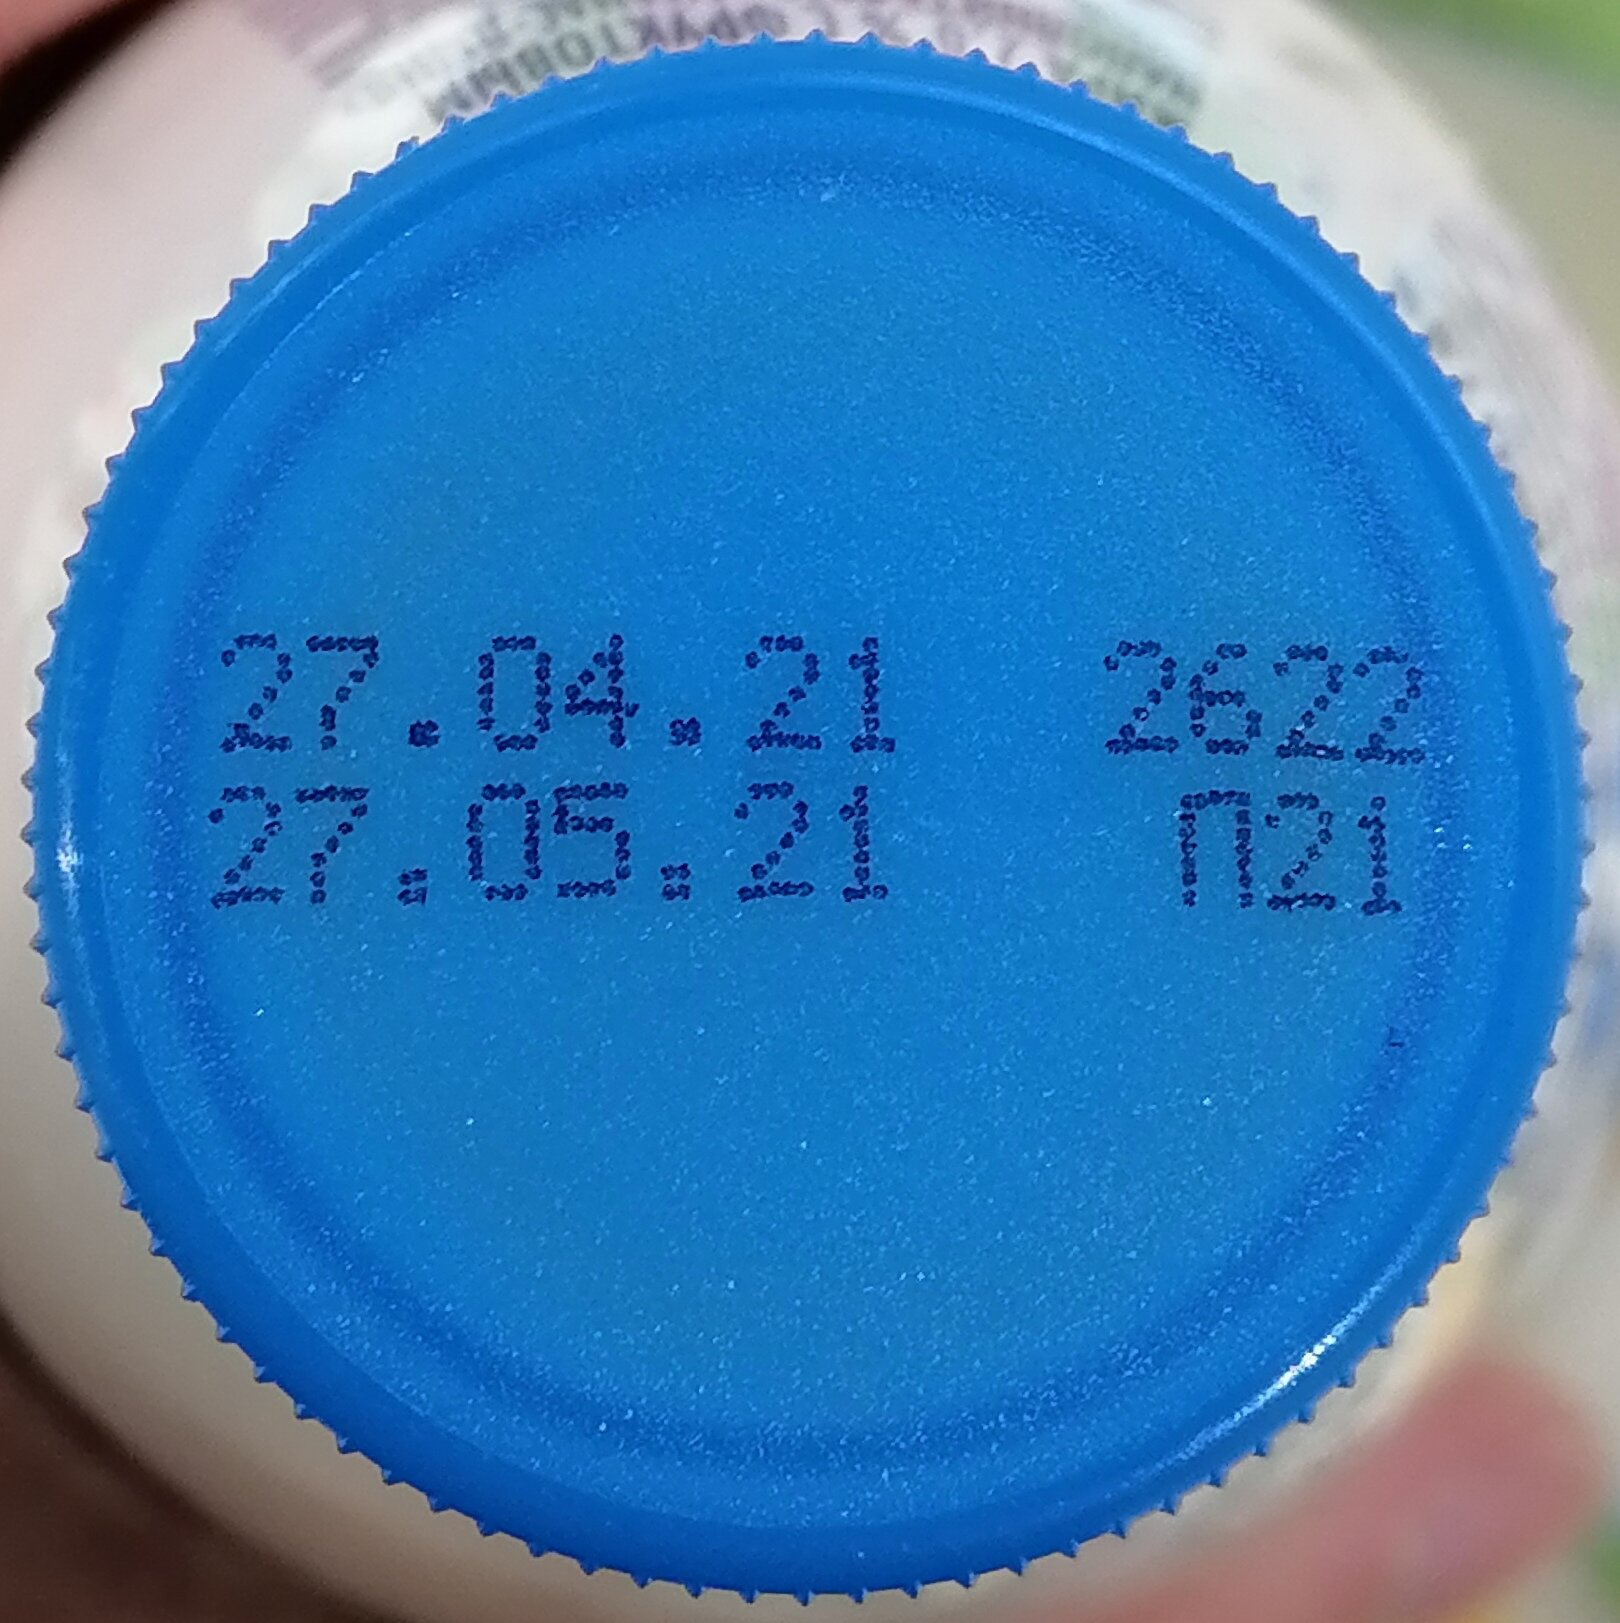
\includegraphics[width=6cm]{man-source/images/ch4/pic4-1.jpg}
	\caption{Продукт с алфавитно-цифровой маркировкой}
	\label{fig:digital_code}
\end{figure}

Важным аспектом является то, что распознавание должно выполняться в реальном времени, основываясь на данных, поступающих с камеры, установленной над производственной линией. Результаты производимого распознавания используются для контроля корректности маркировки.

% Помимо буквенно-цифрового кода (рис. \ref{fig:digital_code}), начиная с недавнего времени, продукция может выпускаться с вариантами маркировки, включающей код Data Matrix (рис. \ref{fig:data_matrix}) \cite{milk}. Данный тип маркировки является удобным и емким представлением специальных и общих данных о продукте. 

% \begin{figure}[ht]
% 	\centering
% 	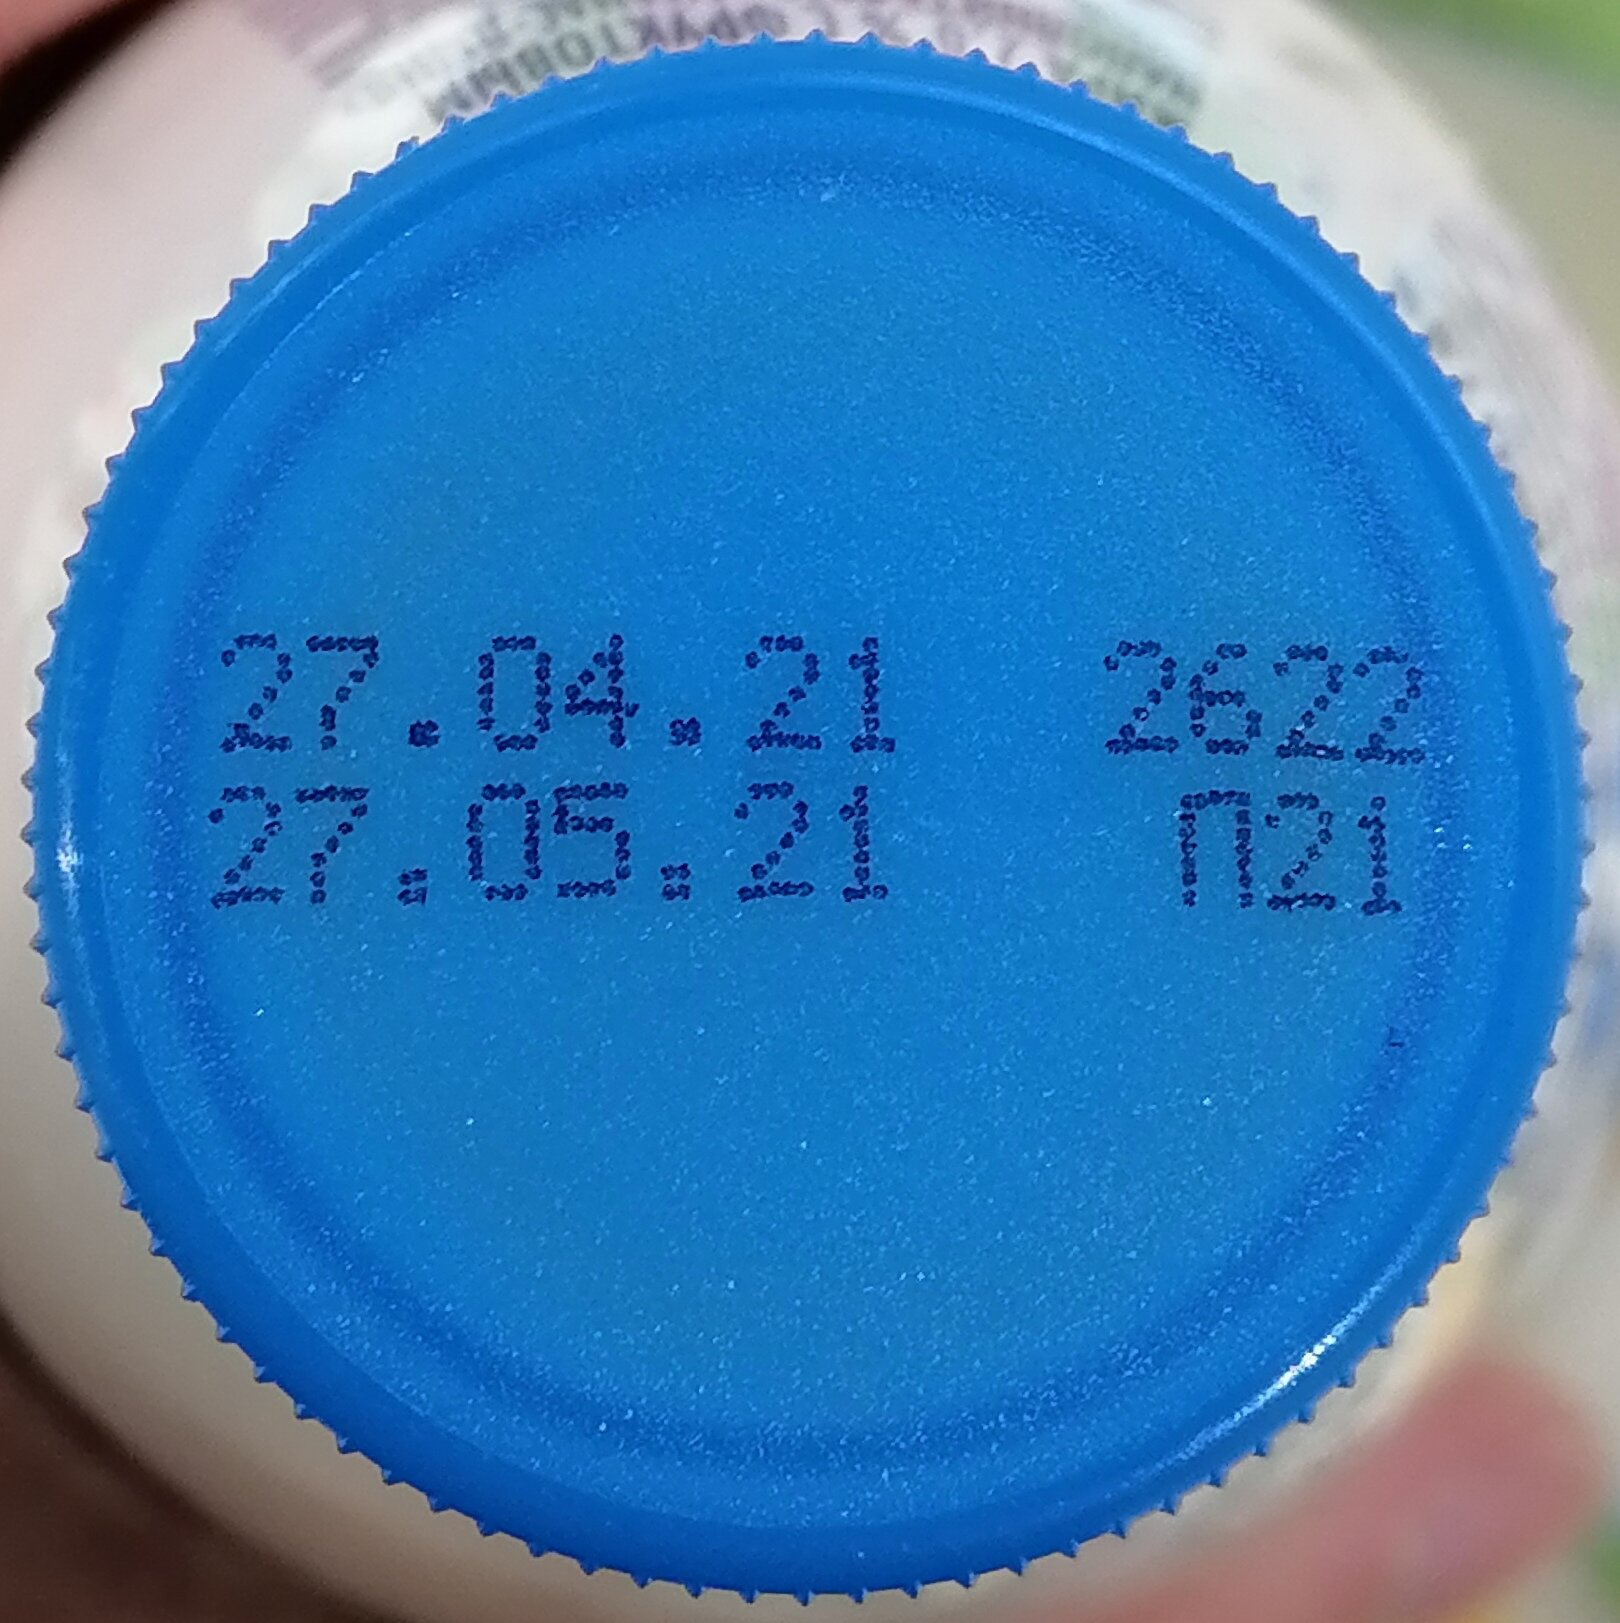
\includegraphics[width=6cm]{man-source/images/ch4/pic4-1.jpg}
% 	\caption{Продукт с буквенно-цифровой маркировкой}
% 	\label{fig:digital_code}
% \end{figure}

% \begin{figure}[ht]
% 	\centering
% 	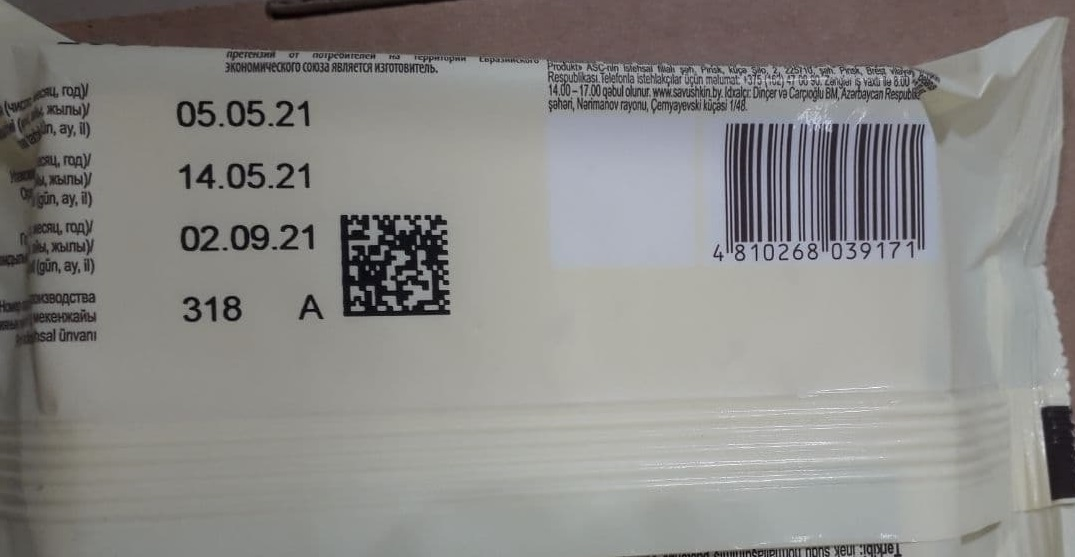
\includegraphics[width=10cm]{man-source/images/ch4/pic4-2.jpg}
% 	\caption{Продукт с кодом Data Matrix}
% 	\label{fig:data_matrix}
% \end{figure}

% Основываясь на общей постановке задачи, были выделены следующие подзадачи, которые должна решать система:
% \begin{easylistNum}
%     & обнаружение и распознавание типа маркировки;
%     & распознавание маркировки;
%     & выявление возможных проблем с маркировкой.
% \end{easylistNum}

К основным проблемам, которые могут возникать в процессе маркирования продуктов, относятся \cite{26-A}:

\begin{easylistNum}
    & \textbf{отсутствие чернил:} в случае поступления на конвейер продуктов без маркировки, система должна сделать вывод об отсутствии чернил, опционально запросив проверку, обратившись к принтеру;
    & \textbf{сдвиг камеры:} если от нейросетевых модулей не поступают данные о результатах распознавания, но системе известно, что движение по конвейеру началось, то она должна сделать вывод о сдвиге камеры;
    & \textbf{ошибочная маркировка:} маркировка была обнаружена и распознана, но не совпала с эталонным представлением. В этом случае должен быть сделан вывод о том, что маркировка неверная;
    & \textbf{нечитаемая маркировка:} в случае, если маркировка получается смазанной и не может быть распознана, необходимо остановить конвейер и сообщить об ошибке оператору.
\end{easylistNum}

Для 1,3 и 4 проблемы необходимо выполнить отсев продуктов, которые имеют ``проблемную'' маркировку. Возникновение этих проблем предполагает полную остановку движения конвейера и сообщение оператору о возникшей проблеме.

Следует отметить, что разработанная система является частью более общей системы, которая используется для анализа и обработки указанных проблем в процессе нанесения маркировки. Общая система реализована с использованием отечественной технологии OSTIS \cite{Golenkov2023}.
%Наша задача заключалась в разработке подсистемы компьютерного зрения для распознавания маркировки продукции.

% Таким образом, резюмируя все вышеназванные задачи и возникающие проблемы, перечислим основные требования, которым должна удовлетворять разрабатываемая система:

% \begin{easylist}
%     & \textbf{Высокая скорость работы}. Конвейер движется очень быстро, поэтому распознавание и анализ должны осуществляться с минимальными задержками;
%     & \textbf{Автономность}. Система должна минимизировать участие оператора;
%     & \textbf{Универсальность}. Система должна настраиваться на распознавание маркировки любой продукции;
%     % & \textbf{Адаптируемость}. Система должна работать при любых условиях, возникающих на производстве (например, недостаточность освещения, ошибки персонала и т.д.).
% \end{easylist}

%Помимо отслеживания маркировки одного лишь человекочитаемого типа (например, буквенно-цифрового), модульная реализация подобных систем позволяет провести универсализацию процесса распознавания и легко добавлять подготовленные модели, осуществляющие распознавание новых типов маркировок, к которым, например, можно отнести код Data Matrix. Такой особый тип матричных штрих-кодов позволяет закодировать специальную идентификационную информацию, а также вес, срок годности, номер серии, номер партии и дату изготовления продукта \cite{datamatrix}.
%Предлагаемая работа посвящена разработке нейросетевого компонента, являющегося частью более общей нейросимволической системы, описанной в \cite{golovko2020}.
Несмотря на существующий интерес к автоматизации производственных процессов и неоспоримые преимущества, которые влечет ее внедрение, подобные задачи решаются в большинстве случаев с участием человека. Оператор периодически выборочно проверяет часть продукции. У такого подхода есть недостатки:

\begin{easylist}
    & есть вероятность того, что будет пропущен момент, когда появится дефект маркировки;
    & скорость реакции человека на возникающую нештатную ситуацию может быть недостаточной;
    & человек может не заметить небольшое расхождение проверяемой маркировки с эталонной (например, в случае ошибочной цифры в дате или номере партии);
    & работа по ручной проверке является монотонной.
\end{easylist}

Существующие аппаратные разработки базируются на использовании специальных датчиков \cite{omron}.

Такие решения осуществляют распознавание маркировки, но имеют ряд важных недостатков:

\begin{easylist}
	& Нестабильное качество распознавания, зависящее от условий, при которых производится съемка (в частности, от освещенности). Так как производственная линия движется быстро, то необходимые условия для качественного распознавания чаще всего не соблюдаются;
	& Необходимость покупки специализированного программного обеспечения для настройки датчиков.
\end{easylist}

Таким образом, появляется необходимость осуществлять контроль за функционированием самой системы распознавания.

В процессе решения указанной задачи были определены факторы, имеющие критическое влияние на процесс решения и подбор алгоритмов:

\begin{easylist}
	& \textbf{Высокая скорость видеопотока}. Так как скорость видеопотока составляет 76 кадров в секунду, то время обработки каждого кадра составляет около 13 миллисекунд. Следует отметить, что этого времени недостаточно для запуска сложной нейросетевой архитектуры, а также для обработки каждого кадра потока.
	& \textbf{Сложность корректной прямой детекции символов (цифр)}. Помимо символов, содержащихся непосредственно в маркировке, в кадр могут попадать символы, нанесенные на другие объекты, например, на сам конвейер или его части. Помимо этого, следует отметить, что изображение попадает на нейронную сеть с уменьшенным разрешением, что приводит к сложности распознавания очень мелких объектов.
\end{easylist}

\subsection{Предлагаемый подход}

Предлагаемый подход состоит в использовании конвейерной структуры из отдельных нейросетевых модулей, каждый из которых решает собственную подзадачу распознавания маркировки.

Задачей данного данного конвейера является обнаружение маркировки, определение ее типа и ее распознавание.

Остановимся далее подробнее на архитектуре системы.

Осуществляя декомпозицию решаемой задачи можно выделить следующие подзадачи:

\begin{easylistNum}
	& Оценка положения товара;
	& Детекция продукта и маркировки;
	& Распознавание частей маркировки;
	& <<Сборка>> маркировки: формирование выходной информации (даты производства товара, номера в партии и т.д.);
	& Проверка распознанной маркировки (определение корректности распознанных данных в соответствии с заранее заданным шаблоном).
\end{easylistNum}

Помимо указанных, в процессе распознавания маркировки решаются дополнительные задачи, связанные с корректностью нанесения такой маркировки.

\begin{easylistNum}
    & определение отсутствия маркировки на продукте;
    & определение наличия искажений маркировки, возникающих в процессе печати, отсутствия ее частей и т.д.
\end{easylistNum}

Указанные задачи решаются в процессе выполнения основных этапов распознавания.

Проблемы, указанные в постановке задачи, решаются архитектурно.

\begin{easylistNum}
    & Высокая скорость видеопотока: решается пропуском незначащих кадров, в которых товар находится не в середине кадра. Это позволяет увеличить интервал времени, необходимый для обработки изображения нейросетью. Оценка значимости осуществляется простой моделью-классификатором с малым временем отработки;
    & Сложность корректной прямой детекции символов: решается осуществлением декомпозиции задачи обнаружения на отдельные подзадачи. В предлагаемой системе в начале обнаруживается товар, затем маркировка на товаре и, наконец, отдельные символы (цифры).
\end{easylistNum}

В предлагаемой нейросетевой системе практически для каждой подзадачи используется отдельная нейросетевая модель, что позволяет легко модифицировать систему, улучшать отдельные модули, изменять их, а также добавлять новые. 

Архитектура системы распознавания представлена на рис. \ref{fig:structure}.

\begin{figure}[!ht]
	\centering
	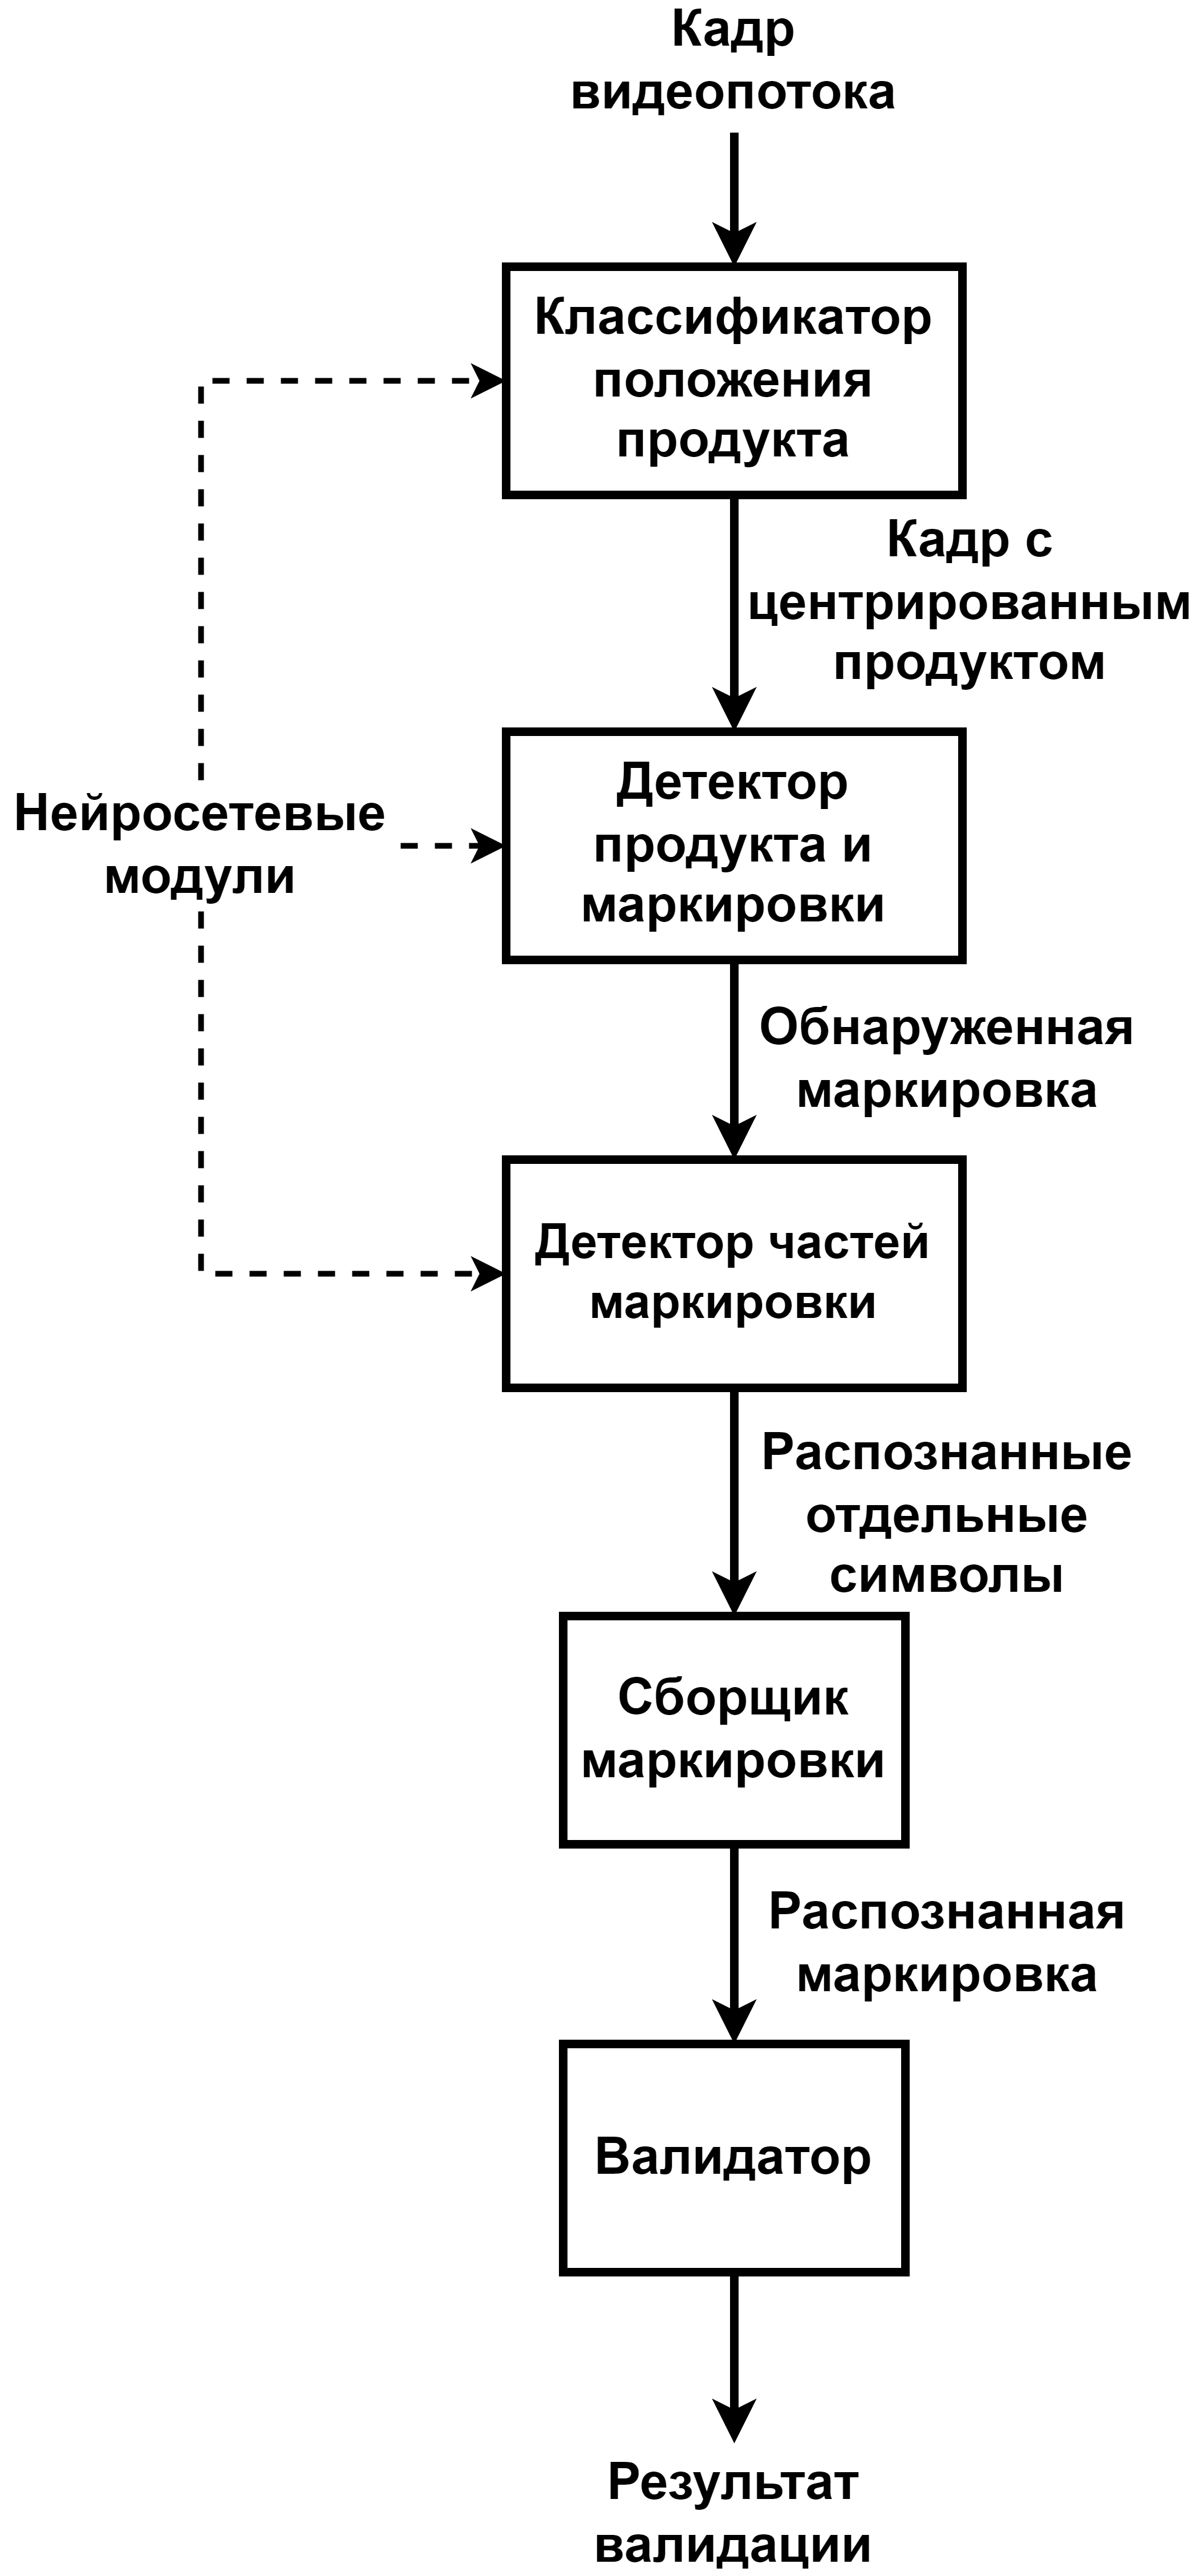
\includegraphics[width=8cm]{man-source/images/ch4/savushkin_structure.png}
	\caption{Структура системы распознавания маркировки}
	\label{fig:structure}
\end{figure}

Опишем основные применяемые нейросетевые модели и их роль в общей архитектуре.

\textbf{Классификатор положения продукта.} Используется предобучаемый сверточный классификатор, который определяет значимость текущего кадра для возможности проведения последующего анализа. При этом наиболее значимым является кадр, в котором товар находится ближе всего к центру кадра (рис. \ref{fig:distance_classes}). Было определено четыре основных класса позиций, по мере удаленности продукта от центра кадра. 1 класс описывает минимальную удаленность. Кадры этого класса участвуют в последующих этапах обработки и анализа. Классы 2 и 3 описывают среднюю и максимальную удаленность. Класс 4 используется для случая отсутствия продукта в кадре (пустая производственная линия).
Кадры, которые идентифицированы как принадлежащие классам 2-4, в дальнейшем анализе не участвуют. 

\begin{figure}[ht]
	\centering
	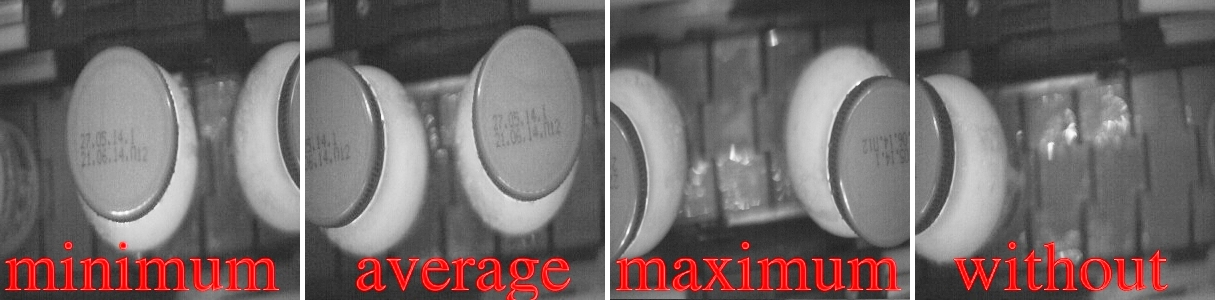
\includegraphics[width=16cm]{man-source/images/ch4/pic4-24.jpg}
	\caption{Примеры изображений разных классов по степени удаленности объекта от центра кадра}
	\label{fig:distance_classes}
\end{figure}

Архитектура применяемого классификатора представлена на рис. \ref{fig:nn_class1}. Он состоит из 5 слоев и имеет 4 выходных нейрона по числу классов, определяющих положение товара в кадре. На всех слоях используется функция активации ReLU за исключением 3-го и последнего слоев. Они используют линейную и softmax-функции активации соответственно. Также применяется max pooling после первого и второго сверточного слоев с параметром stride, равным 2.

\begin{figure}[ht]
	\centering
	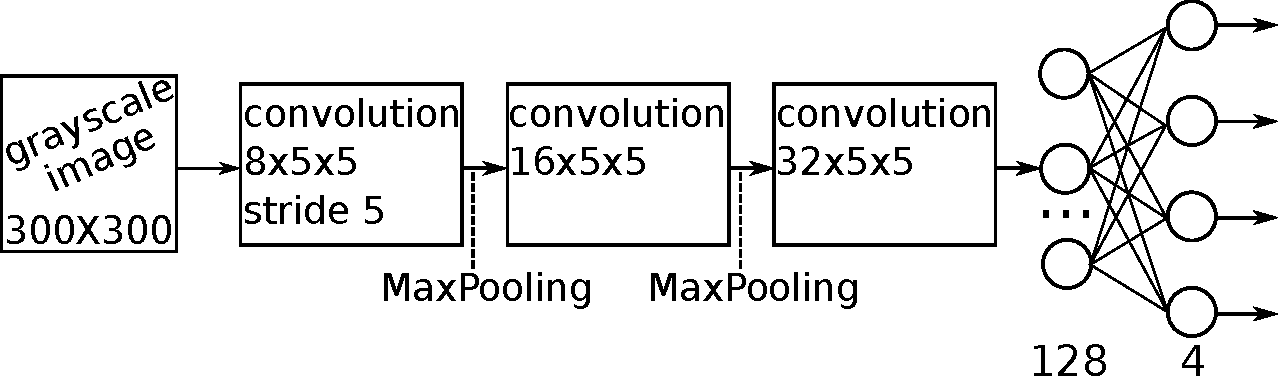
\includegraphics[width=16cm]{man-source/images/ch4/pic4-4.pdf}
	\caption{Структура классификатора для оценки положения бутылки \cite{26-A}}
	\label{fig:nn_class1}
\end{figure}

\textbf{Детектор продукта и маркировки.} Данный детектор осуществляет поиск товара и маркировки в кадре. Здесь в качестве архитектуры была выбрана сеть SSD \cite{liu} на базе классификатора MobileNet v1 \cite{howard}.

Независимое обнаружение товара и маркировки позволяет идентифицировать ситуацию с отсутствующей маркировкой автоматически. Для этого проверяется логическое условие отсутствия маркировки при наличии самого товара в кадре.

Следует отметить, что данный детектор может применяться для обнаружения разных типов маркировки.

В итоге, если маркировка была обнаружена, выполняется передача ее изображения (в оригинальном размере) следующей модели для обработки.

%\textbf{Модуль оценки угла поворота.} В реализации третьего модуля используется регрессор, применяемый для оценки угла поворота маркировки. Данная модель возвращает угол, на который должна быть повернута маркировка для достижения горизонтальной ориентации изображения. Такое преобразование позволяет улучшить качество последующего распознавания цифр. После поворота выполняется передача изображения маркировки на модель для анализа соответствующего типа маркировки (в нашей реализации это модели для анализа кода Data Matrix или цифровой метки).

\textbf{Детектор частей маркировки.} Для анализа алфавитно-цифровой маркировки также используется детектор SSD-MobileNet v1, который осуществляет обнаружение отдельных цифр маркировки.
%Для анализа кода Data Matrix в текущей реализации используется не нейросетевая модель. Применимость нейронной сети для подобного анализа может быть предметом дальнейших исследований.  

После отработки детектора составных частей осуществляется <<сборка>> распознанной маркировки и обработка результата.

Принцип работы нейросетевого компонента на примере алфавитно-цифровой маркировки продемонстрирован на рис. \ref{fig:system_work}.

\begin{figure}[!ht]
	\centering
	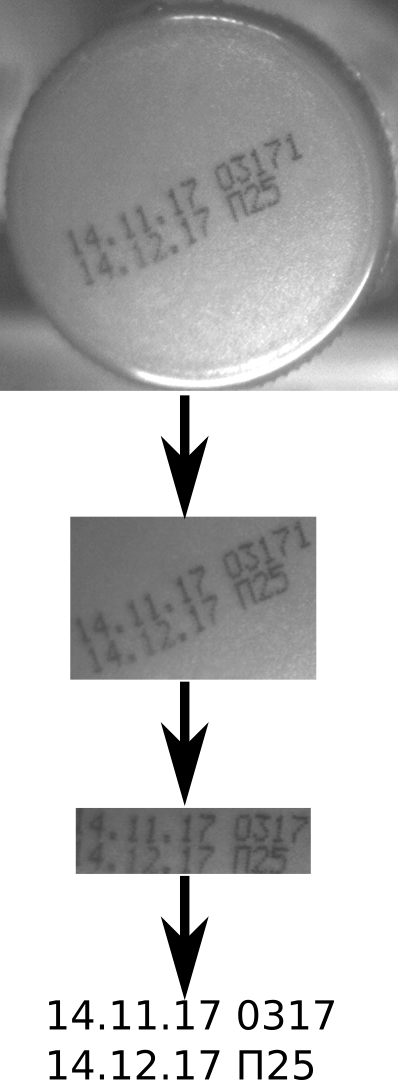
\includegraphics[width=7cm]{man-source/images/ch4/pic4-5.png}
	\caption{Принцип работы системы}
	\label{fig:system_work}
\end{figure}

\subsection{Обучающие выборки: формирование и основные характеристики}

В процессе подготовки нейросетевых моделей использовались различные обучающие выборки:

\begin{easylist}
	& Выборка для обучения классификатора положения;
	& Выборка для обучения детектора маркировок и товаров;
	%& Выборка для обучения регрессора угла поворота
	& Выборка для обучения детектора частей маркировки.
\end{easylist} 

\textbf{Выборка для обучения классификатора положения продукта}. Для создания выборки использовалась модель Faster R-CNN \cite{ren} (на базе  предобученного классификатора ResNet50 \cite{he}). Данная модель обладает лучшими показателями эффективности, чем SSD-MobileNet, но уступает ей в скорости. Она использовалась для автоматической разметки имеющихся данных (главным образом видеофайлов производственного процесса) по степени удаленности товара от центра кадра. В качестве метрики применялось эвклидово расстояние от центра продукта до центра кадра. Таким образом были сформированы четыре класса изображений, которые использовались для последующего обучения сверточного классификатора. Общий объем выборки составил 6189 изображений, 1303 из которых составили тестовую выборку.

\textbf{Выборка для обучения детектора продукта и маркировки}. Для формирования этой выборки использовались размеченные вручную изображения. Общий объем выборки составил 815 изображений, 163 из которых составили тестовую выборку.

%\textbf{Выборка для обучения регрессора угла поворота}. При создании данной выборки использовались изображения маркировок, повернутые под произвольными углами. Общий объем выборки составил 59385 изображений, 11877 из которых составили контрольную выборку. В качестве основы брались изображения маркировок, полученные из выборки для обучения детектора маркировок и товаров.

\textbf{Выборка для обучения детектора частей маркировки}. Для создания этой выборки применялась выборка SVHN \cite{netzer} (выборка номеров домов), а также размеченные цифровые маркировки из уже сформированных выборок. Использовался вариант выборки SVHN, включающий 33402 изображения в обучающей части и 13068 в тестовой (рис. \ref{fig:svhn_dataset}). Объем выборки размеченных цифровых маркировок составил 419 изображений.

\begin{figure}[ht]
	\centering
	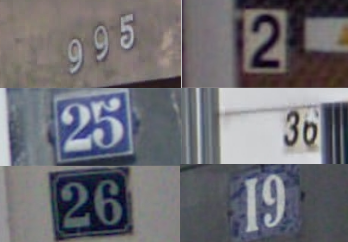
\includegraphics[width=7cm]{man-source/images/ch4/pic4-14.png}
	\caption{Пример изображений из выборки SVHN}
	\label{fig:svhn_dataset}
\end{figure}

\subsection{Результаты обучения и тестирования} 
После обучения классификатора положения продукта итоговая точность распознавания составила \textbf{93.27\%}. Для обучения данной модели применялось предобучение по предлагаемому методу REBA.

Оба детектора (продуктов/маркировок и частей маркировки) обучались на основе предобученных моделей (использовалось предобучение I типа).

Применение SSD-модели позволило достичь эффективности детекции в \textbf{99\% (mAP = 0.99)} для обнаружения товара и маркировки и \textbf{92\% (mAP = 0.92)} для отдельных цифр. Кроме этого, высокая скорость обработки позволила успешно обнаруживать маркировку в видеопотоке. Результаты эффективности распознавания отдельных цифр представлены в таблице \ref{tab:efficiency_detector1}.  

\begin{table}[h]
\caption{Эффективность обнаружения отдельных классов цифр}
\centering
\begin{tabular}{ | c | c |  }
\hline
Class label & AP \\ \hline
0 & 0.9218\\
1. & 0.9107\\
2. & 0.9354\\
3. & 0.9286\\
4. & 0.9265\\
5. & 0.9137\\
6. & 0.9274\\
7. & 0.9167\\
8. & 0.9646\\
9. & 0.8975\\
\hline
\textbf{mAP} & \textbf{0.92429}\\
\hline
\end{tabular}
\label{tab:efficiency_detector1}
\end{table}

Результаты работы детектора продукта и маркировки и детектора частей маркировки изображены на рис. \ref{fig:product_detect}  и \ref{fig:numbers_detect}.

\begin{figure}[!ht]
	\centering
	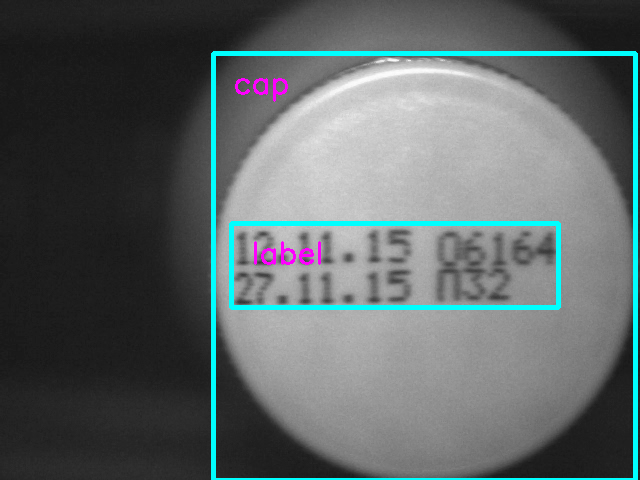
\includegraphics[width=10cm]{man-source/images/ch4/pic4-25.png}
	\caption{Обнаруженный продукт и маркировка}
	\label{fig:product_detect}
\end{figure}

\begin{figure}[!ht]
	\centering
	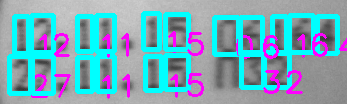
\includegraphics[width=12cm]{man-source/images/ch4/pic4-26.png}
	\caption{Обнаруженные цифры в маркировке}
	\label{fig:numbers_detect}
\end{figure}

Помимо алфавитно-цифровой маркировки (рис. \ref{fig:digital_code}), начиная с недавнего времени, продукция ООО <<Савушкин Продукт>> выпускается с вариантами маркировки, включающей код Data Matrix (рис. \ref{fig:data_matrix}) \cite{milk}. Данный тип маркировки является удобным и емким представлением специальных и общих данных о продукте. 

% \begin{figure}[ht]
% 	\centering
% 	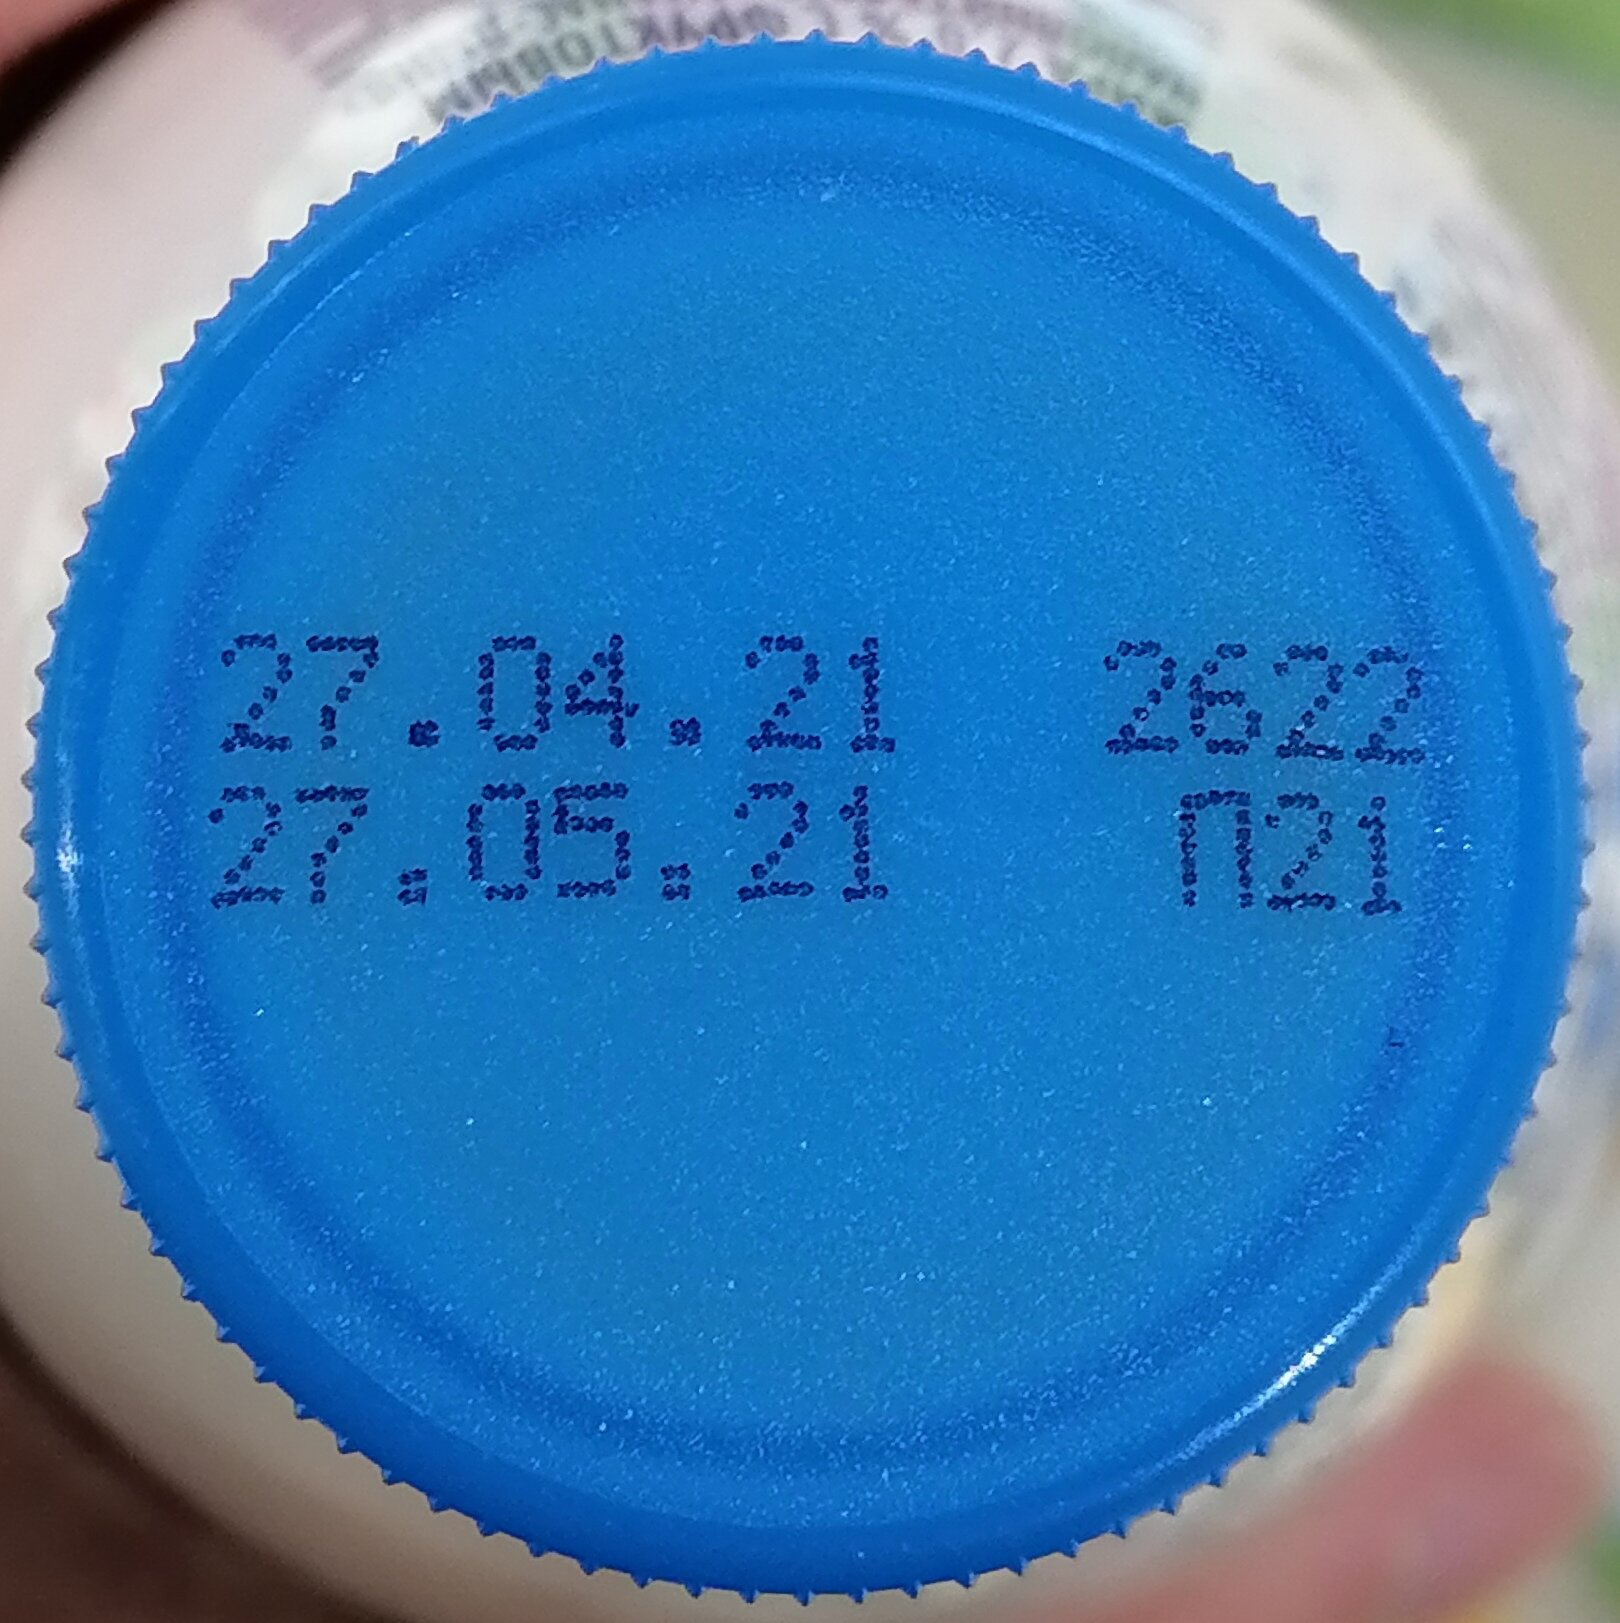
\includegraphics[width=6cm]{man-source/images/ch4/pic4-1.jpg}
% 	\caption{Продукт с буквенно-цифровой маркировкой}
% 	\label{fig:digital_code}
% \end{figure}

\begin{figure}[!ht]
	\centering
	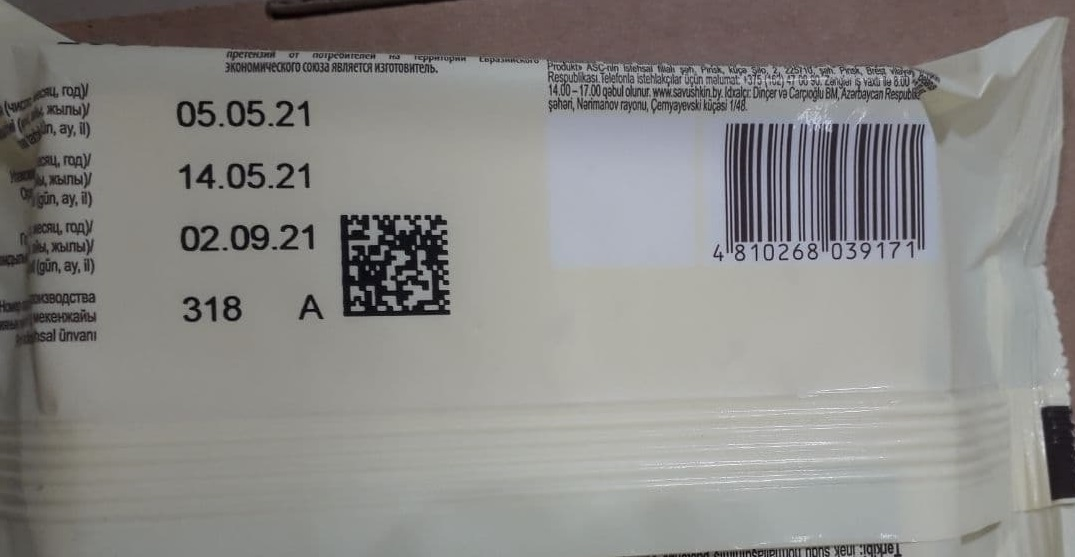
\includegraphics[width=10cm]{man-source/images/ch4/pic4-2.jpg}
	\caption{Продукт с кодом Data Matrix}
	\label{fig:data_matrix}
\end{figure}

Внедрение нового типа маркировки не снижает актуальность предлагаемой разработки, поскольку алфавитно-цифровая маркировка остается единственным вариантом маркировки, который может быть распознан непосредственно человеком. Помимо этого, он продолжает использоваться на всей продукции.

Отметим также, что расширение разработанной системы для обработки новых типов маркировки возможно путем дообучения детектора маркировок на новых данных. Это позволяет гибко расширять систему без необходимости ее повторной реализации.

% \subsection{Заключение}
% В данной работе рассматривается разработка интеллектуального компонента для распознавания маркировки продукции, базирующейся на нейросетевом подходе. Достоинством предложенного решения является использование модульной структуры нейросетевой части, позволяющее осуществлять простую коммутацию между отдельными моделями. Следует отметить универсальность предложенного подхода, которая проявляется в простоте выполнения работы по распознаванию произвольной маркировки на разнообразной продукции. Достаточно интегрировать новый модуль с необходимой функциональностью и система начнет его использовать. Применяемые нами модели отличаются производительностью, благодаря чему возможна работа системы на быстро движущейся производственной линии.

% Направлением дальнейшей работы может быть выбрано улучшение имеющихся результатов распознавания цифровых маркировок, а также исследование применения нейросетевого подхода для распознавания QR-кода.

% \section{Обнаружение и распознавание лиц с функцией дообучения}

%\subsection{Постановка задачи}

%\subsection{Предлагаемый подход}

% Рассмотрим подробнее архитектуру системы компьютерного зрения и принцип действия семантического анализатора. 

% \subsection{Структура модуля компьютерного зрения}

%Модуль компьютерного зрения состоит из последовательности связанных между собой нейросетевых и вспомогательных модулей, используемых для решения задач, которые образуют своеобразный конвейер. %pipeline  

%Связи между этими модулями могут быть организованны как последовательно, так и параллельно. Нейросетевые модули используют нейросетевую модель для решения задачи распознавания, а также выполняют преобразования входных данных модуля во входные данные модели. Вспомогательные модули не используют нейросетевые модели и нужны для преобразования входных данных, выполняемого однократно для нескольких нейросетевых модулей.

%На этапе проектирования конвейера нужно ответить на вопросы, выполняются ли модули параллельно и являются ли выходные данные одного модуля входными данными для другого. Таким образом возникают две топологии -- одна описывает связь модулей с точки зрения параллельности их работы, другая -- с точки зрения передачи входных данных.

%На вход конвейера подается видео-поток, который с помощью вспомогательных модулей разбивается либо на кадры, либо на видеофрагменты. Полученные выходные данные подаются на вход соответствующим веткам конвейера.

%Предложенная модель (\ref{fig:common_arch}) с независимо подключаемыми нейросетевыми модулями позволяет осуществлять параллелизацию вычислений и тем самым уменьшать общее время, затрачиваемое на обработку входных данных. Использование вспомогательных модулей и гибкой настройки связей по входам и выходам позволяет избежать повторной обработки входных данных для различных нейросетевых модулей. 

% Структура разработанного модуля компьютерного зрения представлена на рис. \ref{fig:general_diagram}. Схема сильно упрощена с точки зрения взаимодействия с базой знаний и отражает только последовательность и связанность модулей компьютерного зрения. Рассмотрим данные модули более подробно.

% \begin{figure}[ht]
% 	\centering
% 	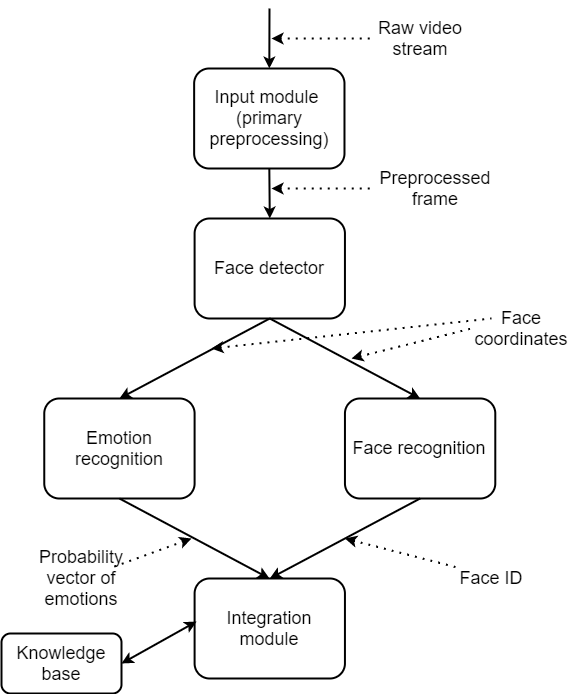
\includegraphics[width=8cm]{man-source/images/ch4/pic4-8.png}
% 	\caption{Конвейер нейросетевых моделей для распознавания маркировки}
% 	\label{fig:general_diagram}
% \end{figure}

% \textbf{Модуль детекции лица} решает задачу обнаружения лиц в кадре. Принимает на вход кадр из видеопотока и возвращает координаты найденных лиц.

% \textbf{Модуль идентификации} нужен для распознавания лица идентифицируемого пользователя. Принимая на вход координаты обнаруженных лиц, данный модуль возвращает идентификаторы пользователей.

% \textbf{Модуль распознавания эмоций} является независимым от логики идентификации. Как и модуль идентификации, принимает на вход координаты обнаруженных лиц и возвращает вероятностный вектор эмоций. 

% После выполнения отдельных веток конвейера, результаты работы модулей передаются на вход интегратора, который выполняет погружение в базу знаний.

% Далее рассмотрим подробнее основные функции модуля компьютерного зрения и полученные результаты при подготовке соответствующих нейросетевых моделей.

% \subsection{Функции модуля компьютерного зрения}

% К функция модуля компьютерного зрения относятся:
% \begin{easylist}
%     & идентификация известного системе пользователя;
%     & идентификация неизвестных пользователей после дообучения; 
%     & распознавание эмоций пользователей.
% \end{easylist}

% \textbf{Идентификация пользователя}. Идентификация пользователя осуществляется модулем идентификации. Наиболее полно процессы, происходящие в модуле, представлены в блок-схеме на рис. \ref{fig:id_flowchart}.

% \begin{figure}[ht]
% 	\centering
% 	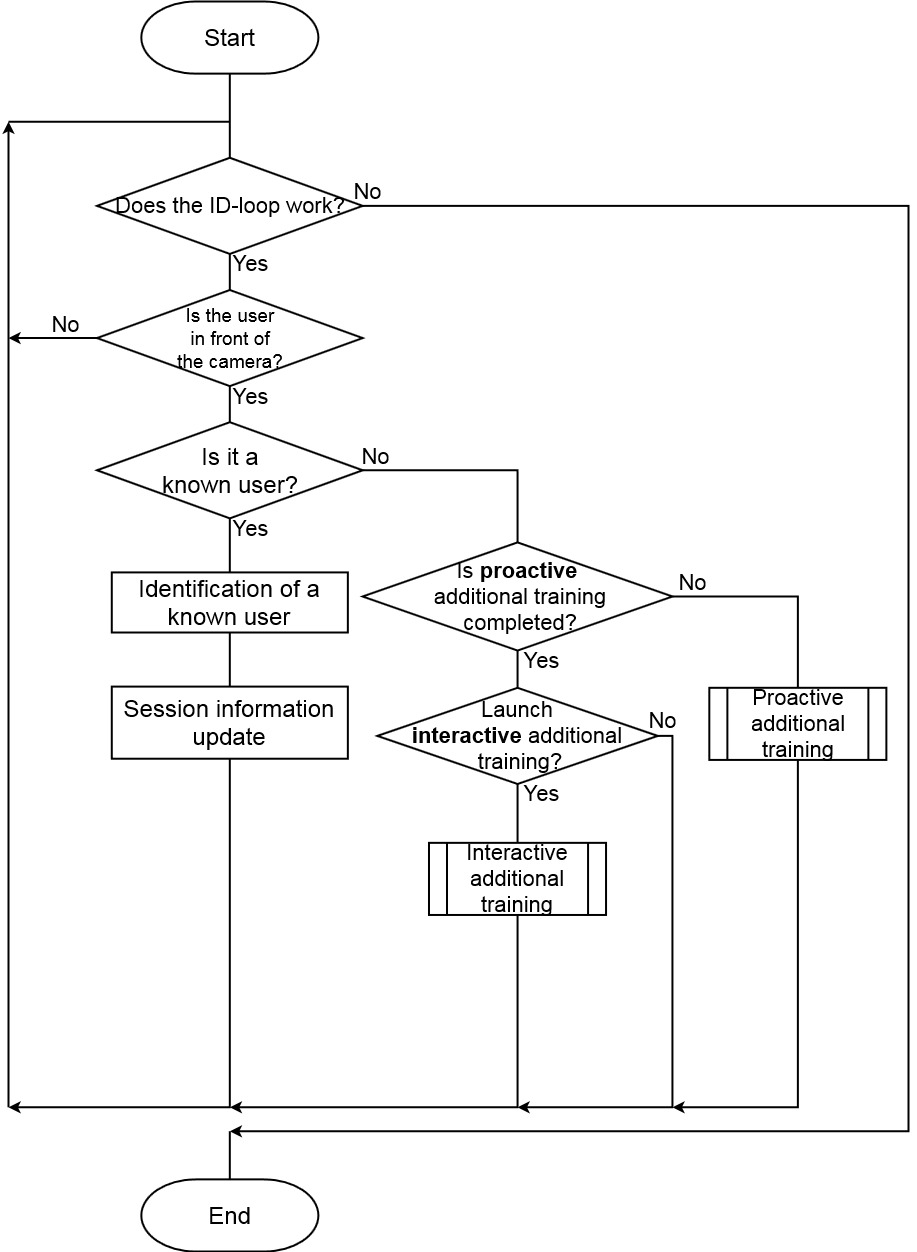
\includegraphics[width=8cm]{man-source/images/ch4/pic4-9.jpg}
% % 	\caption{The overall flowchart of identification}
% 	\caption{Общая блок-схема идентификации}
% 	\label{fig:id_flowchart}
% \end{figure}

% Для реализации данной функции применяется модель нейронной сети FaceNet \cite{facenet}. Для данной модели используются классические модели глубоких сверточных нейронных сетей с триплет-функцией потерь. В нашем случае использовалась сверточная сеть ResNet \cite{resnet}. Общая схема модели представлена на рис. \ref{fig:FaceNet}. 

% \begin{figure}[ht]
% 	\centering
% 	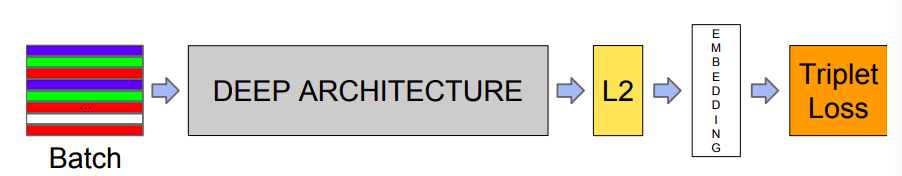
\includegraphics[width=8cm]{man-source/images/ch4/pic4-10.png}
% 	\caption{Структура FaceNet (исходное изображение из \cite{facenet}}
% 	\label{fig:FaceNet}
% \end{figure}

% Данная модель состоит из последовательно идущих слоев глубокой сверточной нейронной сети и $L_2$-нормализации с применением триплет-функции потерь на этапе обучения. На выходе модели формируется 128-размерный вектор признаков, который можно использовать для нативного сравнения лиц.

% В качестве базовой реализации использовались модели из библиотеки dlib \cite{dlib}.

% Рассмотрим алгоритм идентификации пользователя.
% \begin{easylistNum}
% & Лицо пользователя обнаруживается детектором в кадре (в качестве детектора используется модель MTCNN \cite{mtcnn});
% & Для обнаруженного лица осуществляется расчет вектора признаков с помощью ИНС;
% & После вычисления вектора признаков, он сравнивается с другими векторами признаков, сохраненными в базе данных. Данное сравнение выполняется с заданным порогом;
% & На основании результатов, полученных в п. 3, обнаруженному лицу присваивается идентификатор.
% \end{easylistNum}

% Таким образом необходимым условием работы алгоритма является наличие предварительно вычисленных векторов признаков для известных пользователей. Такой подход позволяет с приемлемой скоростью и точностью идентифицировать пользователя.

% Достоинством предложенного подхода является то, что для реализации распознавания не требуется большая обучающая выборка данных, так как используемая модель FaceNet предобучена на большом массиве данных (выборка размером более 3 миллионов изображений) и может использоваться в неизменном виде для идентификации людей, которые не входили в данную выборку.

% Для обучения использовалась выборка фотографий для 7 разных людей, по 7 фотографий каждого человека. Таким образом, объем выборки составил всего 49 фотографий. Для тестирования применялась независимая тестовая выборка из 14 фотографий и набор видеофрагментов, позволяющих оценить качество распознавания пользователей.

% В результате проведения оценки предложенного алгоритма, была получена эффективность распознавания лиц \textbf{95.84\%} в режиме реального времени.

% \textbf{Дообучение для неизвестных пользователей}. Помимо идентификации известных пользователей по векторам признаков, которые присутствуют в базе данных, система позволяет производить дообучение для распознавания незнакомых пользователей в режиме реального времени. Под \textit{дообучением} здесь понимается вычисление набора признаковых векторов для новых пользователей и сохранение их для дальнейшего использования в процессе идентификации. Этот процесс производится в рамках т.н. проактивного и интерактивного дообучения.

% Проактивное дообучение (рис. \ref{fig:proactive_retraining}) производится без прямого участия пользователя, по мере вычисления признаковых векторов на основании кадров, получаемых из видеопотока.

% \begin{figure}[ht]
% 	\centering
% 	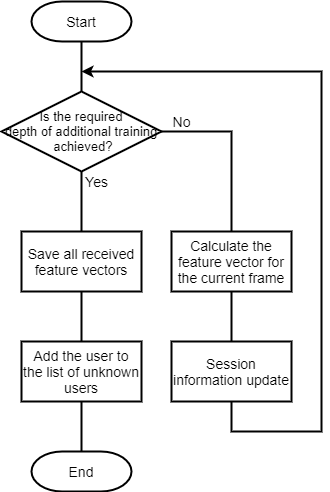
\includegraphics[width=8cm]{man-source/images/ch4/pic4-11.png}
% % 	\caption{The flowchart of proactive additional training}
% 	\caption{Схема проактивного дополнительного обучения}
% 	\label{fig:proactive_retraining}
% \end{figure}

% Интерактивное дообучение для новых пользователей (рис. \ref{fig:interactive_retraining}), проводимое отдельно и с прямым участием пользователя, позволяет улучшить результаты проактивного дообучения и получить более репрезентативные векторы признаков. 

% \begin{figure}[ht]
% 	\centering
% 	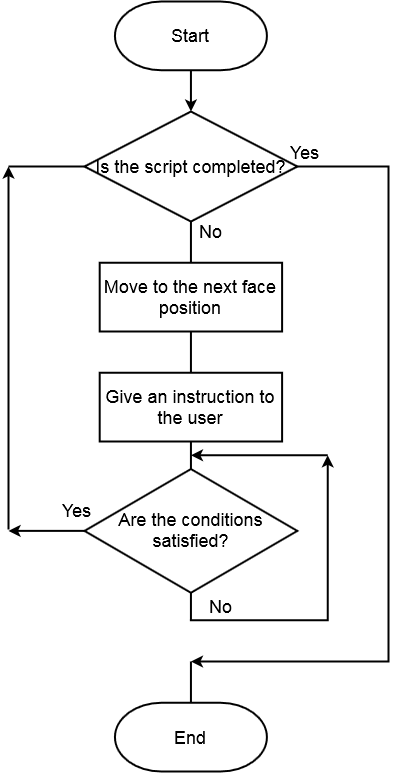
\includegraphics[width=6cm]{man-source/images/ch4/pic4-12.png}
% % 	\caption{The flowchart of interactive additional training}
% 	\caption{Схема интерактивного дополнительного обучения}
% 	\label{fig:interactive_retraining}
% \end{figure}
 
% Рассмотрим алгоритм базового интерактивного дообучения для распознавания новых пользователей:
% \begin{enumerate}
%     \item Пользователь подходит к камере. Осуществляется детекция лица;
%     \item Если это неизвестный пользователь, то после получения согласия от пользователя на выполнение интерактивного дообучения, осуществляется переход на шаг 4. В том случае, если согласия от пользователя получено не было, осуществляется переход на шаг 6;
%     \item Если это известный пользователь, то система приветствует его и осуществляется переход на шаг 6, дообучение в этом случае не производится.

% \textbf{Замечание.} Особый случай составляет ситуация, когда пользователей перед камерой оказывается несколько. Если это так, система идентифицирует неизвестных пользователей (при их наличии) и осуществляет процедуру дообучения персонально, для каждого пользователя;

%     \item Начинается процесс дообучения. Он состоит из последовательного вычисления векторов признаков для различных положений лица в кадре. Основных положений 9: прямо, вверх, вправо вверх, вправо, вправо вниз, вниз, влево вниз, влево, влево вверх. При условии получения согласия от пользователя на сохранение биометрических данных, осуществляется переход на шаг 5, иначе -- осуществляется переход на шаг 6.
%     \item Выполняется сохранение признаковых векторов с идентификатором, присвоенным пользователю, в базе данных.
%     \item Дообучение завершается с выдачей соответствующего сообщения.
% \end{enumerate}

%\subsection{Результаты обучения и тестирования}

\section{Выводы}

\begin{easylistNum}
    & Разработана система определения наличия и детекции солнечных панелей на аэрофотоснимкам. Достоинством разработанной системы является возможность работы системы с фотографиями, имеющими низкое разрешение. Использование предобученных сверточных нейронных сетей позволило достичь точности 87,46 \% в определении наличия солнечных панелей на фото.
	& Разработана система автоматического контроля качества нанесения маркировки продукции. Достоинствами предлагаемого решения является модульная структура, позволяющая осуществлять независимую поддержку каждого функционального модуля. Разработанные нейросетевые модули детекции и распознавания позволили осуществлять обнаружение продукта и его маркировки с эффективностью в \textbf{99\% (mAP = 0.99)} и \textbf{92\% (mAP = 0.92)} для отдельных символов маркировки.
\end{easylistNum}
% \begin{easylist}
%     & ОАО <<Савушкин продукт>> (г. Брест) при разработке решателя задач прототипа системы автоматизации рецептурного производства;
%     & ООО <<ФордэКонсалтинг>> (г. Минск) при разработке решателя задач системы обслуживания клиентов розничной торговли;
%     & ООО <<Кинросс-ресерч>> (г. Минск) при разработке системы автоматизации и оптимизации строительного проектирования;
%     & НИЛ 3.7 при выполнении научно-исследовательской работы БРФФИ--РФФИ <<Формализация темпоральных рассуждений в интеллектуальных системах>> (№ ГР 20164340);
%     & ФГБУН <<Институт систем энергетики им. Л. А. Мелентьева>> СО РАН (г. Иркутск) при разработке решателя задач в области энергетики;
%     & в учебном процессе учреждения образования <<Белорусский государственный университет информатики и радиоэлектроники>>.
% \end{easylist}



% \chapter{РЕАЛИЗАЦИЯ И ПРИМЕНЕНИЕ МОДЕЛЕЙ И СРЕДСТВ ПОСТРОЕНИЯ И МОДИФИКАЦИИ РЕШАТЕЛЕЙ ЗАДАЧ}


% Научные и практические результаты, полученные в рамках данной диссертационной работы, внедрены и используются на следующих предприятиях Республики Беларусь и Российской Федерации:
% \begin{easylist}
%     & ОАО <<Савушкин продукт>> (г. Брест) при разработке решателя задач прототипа системы автоматизации рецептурного производства;
%     & ООО <<ФордэКонсалтинг>> (г. Минск) при разработке решателя задач системы обслуживания клиентов розничной торговли;
%     & ООО <<Кинросс-ресерч>> (г. Минск) при разработке системы автоматизации и оптимизации строительного проектирования;
%     & НИЛ 3.7 при выполнении научно-исследовательской работы БРФФИ--РФФИ <<Формализация темпоральных рассуждений в интеллектуальных системах>> (№ ГР 20164340);
%     & ФГБУН <<Институт систем энергетики им. Л. А. Мелентьева>> СО РАН (г. Иркутск) при разработке решателя задач в области энергетики;
%     & в учебном процессе учреждения образования <<Белорусский государственный университет информатики и радиоэлектроники>>.
% \end{easylist}


% Сведения об использовании результатов диссертационной работы отражены в соответствующих актах внедрения, приведенных в приложении \ref{AppendixActs} к диссертации.

% %\addcontentsline{toc}{chapter}{\introname}	% Добавляем его в оглавление
% \newpage
% \section{Реализация интерпретатора программ языка SCP}

% Для реализации предложенной модели интерпретатора была использована реализация семантической памяти, описанная в \cite{Koronchik2013} и доступная в репозитории \cite{Ostis-dev2017}. Для реализации хранилища sc-текстов использован язык С, разработан собственный формат кодирования sc-текстов и принцип хранения конструкций, внешних по отношению к SC-коду. Кроме того, указанная реализация включает механизм отслеживания событий, необходимый для организации деятельности sc-агентов, а также имеет высокие показатели производительности, что также отражено в упомянутой выше работе. Текущая версия реализации хранилища включает также платформенно-зависимую реализацию описанного ранее механизма блокировок.

% Набор агентов \textit{Абстрактной scp-машины} реализован в виде отдельного программного модуля, входящего в состав указанной реализации платформы интерпретации sc-моделей.

% Указанный модуль имеет двухуровневую архитектуру, обеспечивающую независимость реализации операционной семантики scp-операторов, выполняющих основные преобразования в sc-памяти (нижний уровень) от реализации агентов, которые обеспечивают непосредственно интерпретацию \mbox{scp-операторов} (в том числе -- анализ ролевых отношений, соответствующих scp-операндам), осуществление переходов между ними, создание и удаление scp-процесса и т. д. (верхний уровень). Такая архитектура позволит облегчить внесение корректировок, связанных с возможным изменением в структуре scp-программы или принципах ее интерпретации, в то время как семантика базовых преобразований обусловлена самим языком представления знаний и изменениям практически не подвержена. Нижний уровень предоставляет верхнему набор функций языка С, имеющих унифицированный интерфейс.

% Для обеспечения взаимодействия между уровнями разработан ряд типов данных и структур языка С, соответствующих понятиям предметной области scp-программ. Для обеспечения терминологической совместимости с предыдущими реализациями интерпретатора в программной реализации в ряде случаев сохранены устаревшие имена функций и типов, не всегда очевидно соответствующие современным русскоязычным названиям тех же сущностей.
% Рассмотрим подробнее разработанные типы и структуры данных.
% Перечисление (enumeration), описывающее классификацию scp-операндов по фиксированности/нефиксированности значения:

% \begin{lstlisting}[style={CppCodeStyle}]
% enum _scp_param_type
% {
%     SCP_ASSIGN = 0, // scp-операнд со свободным значением'
%     SCP_FIXED = 1 // scp-операнд с фиксированным значением'
% };
% typedef enum _scp_param_type scp_param_type;

% \end{lstlisting}

% Перечисление (enumeration), описывающее классификацию \mbox{scp-операндов} по константности/переменности:

% \begin{lstlisting}[style={CppCodeStyle}]
% enum _scp_operand_type
% {
%     SCP_CONST = 0, // scp-константа'
%     SCP_VAR = 1 // scp-переменная'
% };
% typedef enum _scp_operand_type scp_operand_type;
% \end{lstlisting}

% Перечисление (enumeration), описывающее возможные результаты выполнения того или иного scp-оператора, в зависимости от чего осуществляется переход к следующему оператору:

% \begin{lstlisting}[style={CppCodeStyle}]
% enum _scp_result
% {
%     SCP_RESULT_FALSE = 0, // успешное выполнение
%     SCP_RESULT_TRUE = 1, // безуспешное выполнение
%     SCP_RESULT_ERROR // выполнение с ошибкой
% };
% typedef enum _scp_result scp_result;
% \end{lstlisting}

% Типы языка C, соответствующие ролевым отношениям, уточняющим тип sc-элемента, являющегося значением scp-переменной:

% \begin{lstlisting}[style={CppCodeStyle}]
% typedef sc_uint16 scp_type;

% extern scp_type scp_type_node; //sc-узел
% extern scp_type scp_type_arc; //sc-дуга
% extern scp_type scp_type_link; //sc-ссылка
% extern scp_type scp_type_edge_common; //sc-ребро общего вида
% extern scp_type scp_type_arc_common; //sc-дуга общего вида
% extern scp_type scp_type_arc_access; //sc-дуга принадлежности

% extern scp_type scp_type_const; //sc-константа
% extern scp_type scp_type_var; //sc-переменная

% extern scp_type scp_type_arc_pos; //позитивная sc-дуга принадлежности
% extern scp_type scp_type_arc_neg; //негативная sc-дуга принадлежности
% extern scp_type scp_type_arc_fuz; //нечеткая sc-дуга принадлежности

% extern scp_type scp_type_arc_temp; //нестационарная sc-дуга принадлежности
% extern scp_type scp_type_arc_perm; //стационарная sc-дуга принадлежности

% extern scp_type scp_type_arc_pos_const_perm; //константная позитивная стационарная sc-дуга принадлежности

% extern scp_type scp_type_node_not_binary_tuple; //знак связки 
% extern scp_type scp_type_node_struct; //знак структуры
% extern scp_type scp_type_node_role_relation; //знак ролевого отношения
% extern scp_type scp_type_node_norole_relation; //знак неролевого отношения
% extern scp_type scp_type_node_not_relation; //знак класса
% extern scp_type scp_type_node_abstract; //знак абстрактной сущности
% extern scp_type scp_type_node_material; //знак материальной сущности

% \end{lstlisting}


% Перечисление (enumeration), описывающее признак наличия того или иного свойства у scp-операнда (стандартный тип языка С не используется во избежание потенциальных проблем с последующей аппаратной реализацией платформы и интерпретатора):

% \begin{lstlisting}[style={CppCodeStyle}]
% enum _scp_bool
% {
%     SCP_FALSE = 0,
%     SCP_TRUE = 1
% };
% typedef enum _scp_bool scp_bool;
% \end{lstlisting}

% Структура языка C, описывающая конкретный scp-операнд с учетом всех специфицирующих его ролевых отношений:

% \begin{lstlisting}[style={CppCodeStyle}]
% struct _scp_operand
% {
%     sc_addr addr; // физический адрес соответствующего sc-элемента
%     scp_param_type param_type; // фиксированность/нефиксированность
%     scp_type element_type; // тип sc-элемента
%     scp_operand_type operand_type; // scp-константа/scp-переменная
%     scp_bool erase; // признак удаления sc-элемента (для scp-операторов удаления)
%     scp_bool set; // признак множества (для scp-операторов поиска с формированием множеств)
% };

% typedef struct _scp_operand scp_operand;

% \end{lstlisting}

% Структура языка C, описывающая пару scp-операндов (используется, например, в scp-операторе поиска конструкций по произвольному образцу для задания ограничений поиска):


% %listing
% \begin{lstlisting}[style={CppCodeStyle}]
% struct _scp_operand_pair
% {
%     scp_operand *operand1;
%     scp_operand *operand2;
% };
% typedef struct _scp_operand_pair scp_operand_pair;

% \end{lstlisting}


% Пример заголовка функции, реализующей scp-оператор поиска трехэлементной конструкции:

% \begin{lstlisting}[style={CppCodeStyle},breaklines=true]
% scp_result searchElStr3(sc_memory_context *context, scp_operand *param1, scp_operand *param2, scp_operand *param3);

% \end{lstlisting}
% \newpage
% \section{Реализация системы автоматизации процесса построения и модификации решателей задач}

% Текущая версия системы автоматизации процесса построения и модификации решателей задач реализована в соответствии с представленной выше моделью и использованием предложенных в данной работе моделей и средств.

% Агенты системы реализованы с использованием языка SCP. В настоящий момент \textit{Решатель задач системы автоматизации процесса построения и модификации решателей задач} имеет в своем составе 22 агента.

% Пользовательский интерфейс системы автоматизации процесса построения и модификации решателей задач построен на основе существующей реализации платформы интерпретации sc-моделей интерфейса, доступной в репозитории \cite{SC-WEB2017}. Указанная реализация выполнена в web-ориентированном варианте, таким образом, доступ к системе осуществляется посредством \mbox{web-браузера}. Такой вариант реализации позволяет работать с системой удаленно, в том числе осуществлять коллективную работу, при этом не требуется никаких дополнительных средств, кроме обычного браузера, входящего в состав любой современной операционной системы, в том числе операционных систем для мобильных устройств.

% Указанная реализация ориентирована на работу с рассмотренной выше версией реализации семантической памяти и в комплексе с ней в настоящее время используется в качестве основного варианта реализации \textit{платформы интерпретации sc-моделей}, используемого в рамках технологии OSTIS на текущем этапе развития.

% Рассмотрим примеры работы системы автоматизации процесса построения и модификации scp-программ.

% Добавление точки останова в тестовую программу (рисунок~\ref{fig:pic4_1}):
% \begin{figure}[H]
%     \centering
%     \includegraphics{man-source/images/ch4/pic4_1.png}
%     \caption{Добавление точки останова}
%     \label{fig:pic4_1}
% \end{figure}


% После запуска программы на тестовых данных выполнение соответствующего процесса остановлено при достижении указанной ранее точки останова. Пользователь выполняет поиск оператора, на котором остановлено выполнение (рисунок~\ref{fig:pic4_2}):
% \begin{figure}[H]
%     \centering
%     \includegraphics{man-source/images/ch4/pic4_2.png}
%     \caption{Поиск остановленных операторов}
%     \label{fig:pic4_2}
% \end{figure}


% Оператор найден (рисунок~\ref{fig:pic4_3}):
% \begin{figure}[H]
%     \centering
%     \includegraphics{man-source/images/ch4/pic4_3.png}
%     \caption{Оператор, на котором остановилось выполнение отлаживаемого процесса}
%     \label{fig:pic4_3}
% \end{figure}

% Далее, используя стандартные средства навигации, пользователь может просмотреть состояние памяти в окрестности остановленного оператора, например, просмотреть значения его операндов (рисунок~\ref{fig:pic4_4}):
% \begin{figure}[H]
%     \centering
%     \includegraphics{man-source/images/ch4/pic4_4.png}
%     \caption{Запрос семантической окрестности оператора}
%     \label{fig:pic4_4}
% \end{figure}


% Семантическая окрестность остановленного оператора (рисунок~\ref{fig:pic4_5}):
% \begin{figure}[H]
%     \centering
%     \includegraphics{man-source/images/ch4/pic4_5.png}
%     \caption{Семантическая окрестность оператора}
%     \label{fig:pic4_5}
% \end{figure}

% Далее выполнение процесса может быть продолжено в режиме пошагового выполнения или до конца процесса.

% Как видно из приведенных примеров, спроектированная и реализованная система автоматизации процесса построения и модификации scp-программ обладает всей базовой функциональностью современных сред проектирования программ, таким как возможность использования точек останова и пошагового выполнения. При этом средства навигации в составе описанной системы позволяют просматривать любую информацию в окрестности остановленного процесса, в том числе -- значения переменных, а также позволяют отслеживать изменения, происходящие в памяти. Кроме того, по аналогии с современными средами рассматриваемая система содержит средства автоматической верификации проектируемых программ.
% \newpage
% \section{Вклад в развитие технологии OSTIS} \label{section_contrib}

% Все предложенные в рамках данной работы модели и средства формально описаны, включены в состав соответствующих разделов базы знаний метасистемы IMS и доступны на сайте \cite{IMS2017}.
% Перечислим явно разделы базы знаний IMS, разработанные в рамках данной диссертационной работы:

% \begin{easylist}
% & \textit{Раздел. Предметная область действий и задач} (раздел \ref{section_actions});

% & \textit{Раздел. Предметная область действий, выполняемых в семантической памяти ostis-системы (действий в sc-памяти)} (подраздел \ref{section_actions_in_sc_memory});

% & \textit{Раздел. Предметная область агентов, работающих в семантической памяти ostis-системы (sc-агентов)} (разделы \ref{section_agents}, \ref{section_sync});

% & \textit{Раздел. Предметная область действий и спецификаций действий базовой машины обработки унифицированных семантических сетей (Абстрактной scp-машины)} (раздел \ref{section_scp});

% & \textit{Раздел. Предметная область агентов абстрактной scp-машины и соответствующих им микропрограмм} (раздел \ref{section_scp_interpreter});

% & \textit{Раздел. Предметная область действий разработчиков машин обработки знаний} (разделы \ref{section_method_1}, \ref{section_method_2});

% & \textit{Библиотека многократно используемых компонентов абстрактных \mbox{sc-машин}} (раздел \ref{section_library});

% & \textit{Раздел. Подсистема поддержки проектирования sc-агентов} (\mbox{раздел \ref{section_tools}});

% & \textit{Раздел. Подсистема поддержки проектирования программ базового языка программирования Технологии OSTIS} (раздел \ref{section_tools}).

% \end{easylist}

% Кроме того, внесен вклад в развитие библиотек многократно используемых компонентов, входящих в состав IMS и представленных в рамках \textit{Раздела. Библиотека многократно используемых компонентов абстрактных sc-машин} и его подразделов.

% Текущая версия \textit{Библиотеки многократно используемых абстрактных sc-агентов} содержит:
% \begin{easylist}
% &	28 агентов информационного поиска;
% &	6 агентов верификации баз знаний;
% &	5 агентов редактирования баз знаний.

% \end{easylist}

% Текущая версия \textit{Библиотеки многократно используемых scp-программ} содержит 10 scp-программ (без учета scp-программ, соответствующих указанным выше агентам).

% Реализация системы автоматизации процесса построения и модификации решателей задач включена в состав \textit{Библиотеки типовых подсистем ostis-систем}.

% \newpage
% \section{Применение разработанных моделей и средств}

% Первоначальное применение разработанных моделей и средств осуществлялось в рамках самой метасистемы поддержки проектирования интеллектуальных систем IMS \cite{IMS2017,Golenkov2014b}.

% Кроме того, результаты диссертационной работы использованы для построения объединенных решателей задач интеллектуальных справочных систем (ИСС) по различным предметным областям.

% Наибольший интерес представляют прототипы решателей задач ИСС по геометрии Евклида и ИСС по теории графов. Это обусловлено, во-первых, относительной развитостью и сложностью указанных прототипов, а во-вторых, тем, что указанные системы используют принципиально разные подходы к решению задач. 

% В рамках ИСС по геометрии Евклида реализованы стратегия поиска решения задачи в глубину и механизм прямого логического вывода на основе продукций, позволяющие решать задачи в несколько действий, используя логические утверждения (теоремы, аксиомы) вида <<ЕСЛИ--ТО>>, хранящиеся в базе знаний, путем применения правила modus ponens.

% В свою очередь, в рамках ИСС по теории графов реализуется концепция пакета программ, в основе которой лежит механизм сведения задачи к подзадачам, каждая из которых в конечном итоге решается путем выполнения хранимой в памяти системы программой на некоторых входных данных. Указанный механизм также позволяет решать задачи в несколько действий, т. е. такие задачи, для которых нет заранее заготовленной программы, с помощью которой можно было бы решить данную задачу.

% Кроме того, объединенный решатель задач каждого из рассматриваемых прототипов имеет в своем составе набор поисковых агентов, многие из которых были заимствованы из библиотеки многократно используемых sc-агентов, а некоторые реализованы специально для соответствующей системы, поскольку являются предметно-зависимыми.

% \subsection{Оценка эффективности предложенных методики и библиотеки} \label{section_effect}

% Как показывает результат анализа процесса разработки указанных систем, а также ряда других, предложенные в работе модель решателя задач и методика их построения и модификации позволяют в высокой степени унифицировать и универсализировать различные компоненты решателя. Так, для разработки прототипа ИСС по некоторой предметной области, позволяющего осуществлять простейшую навигацию по базе знаний, может без каких-либо дополнений использоваться готовый коллектив агентов информационного поиска, входящий в состав соответствующей библиотеки. Кроме того, реализованные для ИСС по геометрии и теории графов решатели задач также могут быть использованы в других системах, поскольку не ориентированы на какую-либо конкретную предметную область.

% Так, например, приведем список, отражающий число агентов, реализованных для перечисленных систем (без учета уже готовых, заимствованных из библиотеки) с указанием числа агентов, включенных в состав соответствующих библиотек:

% \begin{easylist}
% &	объединенный решатель задач системы поддержки проектирования решателей задач -- 13 агентов (включены в библиотеку в составе указанной системы);
% &	объединенный решатель задач IMS -- 10 агентов информационного поиска (все включены в состав соответствующей библиотеки);
% &	объединенный решатель задач ИСС по геометрии Евклида -- 17 агентов информационного поиска (все включены в состав соответствующей библиотеки), 10 атомарных агентов в составе решателя задач (все включены в состав соответствующей библиотеки), заимствовано из библиотеки 10 агентов информационного поиска;
% &	объединенный решатель задач ИСС по теории графов -- 17 специализированных агентов, 5 атомарных агентов в составе решателя, 25 агентов заимствовано из библиотеки.
% \end{easylist}

% Как видно из приведенного списка, разработка каждой следующей системы существенно упрощается за счет использования готовых универсальных компонентов. Число агентов, заимствованных из библиотеки в процессе разработки ИСС по теории графов показывает, что уже текущий вариант наполнения библиотеки позволяет составить из готовых компонентов существенную часть разрабатываемого решателя. В дальнейшем планируется активное пополнение библиотек новыми компонентами.

% С течением времени и развитием решателей задач количество таких компонентов будет увеличиваться, что, соответственно, будет приводить к еще большему показателю заимствования. Для определения снижения временных затрат за счет заимствования на данный момент развития библиотеки был использован пессимистический подход, предполагающий оценку наименьшего заимствования в существующих на сегодня системах. 

% Для оценки временных затрат на разработку решателей была выделена условная классификация агентов по сложности, предполагающая, что на разработку агентов каждого класса затрачивается примерно одно время, включающее в себя время на собственно реализацию агента и время на его отладку. 

% К таким классам относятся:

% \begin{easylist}
% & поисковый агент (поиск всех элементов заданного множества, поиск всех идентификаторов заданной сущности и т. д.);
% & усложненный поисковый агент (поиск семантической окрестности заданной сущности, поиск всех сущностей, являющихся частными/общими по отношению к заданной сущности и т. д.);
% & агент логического вывода;
% & агент расчета операций (арифметических, теоретико-множественных, операций на матрицах и векторах и т. д.).
% \end{easylist}

% В таблице \ref{TimeNormTable} приведены данные о времени на реализацию и отладку агентов каждого класса. Указанные данные основаны на результатах анализа фактических затрат времени на разработку агентов решателя задач.

% \begin{table} [H]
%   \small
%   \caption{Средняя продолжительность разработки агентов}\label{TimeNormTable}
% \begin{tabularx}{\hsize}{| X | X | X | X |}
%   \hline
%  \multirow{2}{*}{Тип агента} &\multicolumn{2}{c|}{Длительность операции, ч } & \multirow{2}{*}{Всего, ч}\\
%  \cline{2-3}
%   & Реализация агента & Отладка агента & \\
% \hline
 
% Поисковый агент	& 1,5	& 0,5	& 2\\
% \hline
% Усложненный поисковый агент	& 8	& 3	& 11\\
% \hline
% Агент логического вывода	& 12	& 4	& 16\\
% \hline
% Агент расчета операций	& 6	& 2	& 8\\
% \hline
% \end{tabularx}
% \end{table}

% Как видно из таблицы, временные затраты на разработку поискового агента составляют 2 ч, усложненного поискового агента – 11 ч, агента логического вывода – 16 ч, агента расчета операций – 8 ч.
% В таблице \ref{AgentsCountTable} приведено количество агентов, входящих в каждый отдельный решатель, а также количество заимствованных агентов в каждом решателе. 

% \begin{table} [H]
%   \small
%   \caption{Количество агентов в решателях}\label{AgentsCountTable}
% \begin{tabularx}{\hsize}{| p{2.5cm} | X | X | X | X | X | X | X |}
%   \hline
%  \multirow{2}{*}{Тип агента} &\multicolumn{7}{c|}{Количество агентов, шт.}\\
%  \cline{2-8}
%  & ИСС по теории множеств & ИСС по числовым моделям	& ИСС по истории	& ИСС по химии	& ИСС по географии	& Система автоматизации предприятия	& Система обслуживания розничной торговли\\
% \hline
% Поисковые агенты,  & 9 & 15 & 12 & 10 & 11 & 12 & 9\\
% \cline{2-8}
% в том числе заимствованных & 7 & 8 & 7 & 6 & 7 & 10 & 5\\
% \hline
% Усложнен-ные поисковые агенты, & 5 & 11 & 13 & 5 & 5 & 6 & 6\\
% \cline{2-8}
% в том числе заимствованных & 3 & 5 & 5 & 3 & 3 & 3 & 3\\
% \hline
% Агенты \mbox{логического} вывода, & 1 & 3 & 4 & 3 & 1 & 0 & 0\\
% \cline{2-8}
% в том числе заимствованных & 0 & 0 & 1 & 1 & 0 & 0 & 0\\
% \hline
% Агенты расчета операций, & 8 & 20 & 3 & 10 & 6 & 4 & 2\\
% \cline{2-8}
% в том числе заимствованных & 5 & 5 & 1 & 4 & 0 & 1 & 0\\
% \hline
% Итого  & 23 & 49 & 32 & 28 & 23 & 22 & 17\\
% \hline
% Итого заимствованных & 15 & 18 & 14 & 14 & 10 & 14 & 8\\
% \hline

% \end{tabularx}
% \end{table}

% На основе данных, представленных в таблицах \ref{TimeNormTable} и \ref{AgentsCountTable}, определена продолжительность разработки агентов для каждой из представленных систем по формуле (\ref{eq_agent_1}):

% \begin{equation}
%     \label{eq_agent_1} 
%     t_{cj} = \sum_{i=1}^{m} t_{aj} \cdot N_i,	
% \end{equation}
% где $t_{cj}$ – продолжительность разработки всех агентов для решателя \textit{j}-й системы (ч);

% \parindent=8mm
% $t_{aj}$ – продолжительность разработки агента \textit{i}-го типа (ч);

% \textit{m} – количество типов агентов, входящих в систему \textit{j} (шт.);

% $N_i$ – количество агентов \textit{i}-го типа в \textit{j}-й системе (шт.).
% \parindent=10mm

% Результаты расчетов сведены в таблицу \ref{AgentsTimeTable}.

% \begin{table} [H]
%   \small
%   \caption{Расчет временных затрат на разработку агентов}\label{AgentsTimeTable}
% \begin{tabularx}{\hsize}{| p{2.5cm} | X | X | X | X | X | X | X |}
%   \hline
%  \multirow{2}{*}{Тип агента} &\multicolumn{7}{c|}{Продолжительность разработки агентов, ч}\\
%  \cline{2-8}
%  & ИСС по теории множеств & ИСС по числовым моделям	& ИСС по истории	& ИСС по химии	& ИСС по географии	& Система автоматизации предприятия	& Система обслуживания розничной торговли\\
% \hline
% Поисковые агенты,  & 18 & 30 & 24 & 20 & 22 & 24 & 18\\
% \cline{2-8}
% в том числе заимствованных & 14 & 16 & 14 & 12 & 14 & 20 & 10\\
% \hline
% Усложнен-ные поисковые агенты, & 55 & 121 & 143 & 55 & 55 & 66 & 66\\
% \cline{2-8}
% в том числе заимствованных & 33 & 55 & 55 & 33 & 33 & 33 & 33\\
% \hline
% Агенты \mbox{логического} вывода, & 16 & 48 & 64 & 48 & 16 & 0 & 0\\
% \cline{2-8}
% в том числе заимствованных & 0 & 0 & 16 & 16 & 0 & 0 & 0\\
% \hline
% Агенты расчета операций, & 64 & 160 & 24 & 80 & 48 & 32 & 16\\
% \cline{2-8}
% в том числе заимствованных & 40 & 40 & 8 & 32 & 0 & 8 & 0\\
% \hline
% Итого  & 153 & 359 & 255 & 203 & 141 & 122 & 100\\
% \hline
% Итого заимствованных & 87 & 111 & 93 & 93 & 47 & 61 & 43\\
% \hline

% \end{tabularx}
% \end{table}

% Таким образом, использование методики построения и модификации решателей задач с применением многократно используемых компонентов позволяет сократить время разработки каждого решателя на время разработки заимствованных агентов. 
% Удельный вес продолжительности разработки заимствованных агентов в общем времени разработки общего числа агентов для каждого решателя можно определить по формуле (\ref{eq_agent_2}):

% \begin{equation}
%     \label{eq_agent_2} 
%     SW_{lj} = \frac{t_{lj} \cdot 100~\%}{t_{cj}},	
% \end{equation}
% где $SW_{lj}$ –удельный вес продолжительности разработки заимствованных агентов в общем времени разработки общего числа агентов для \textit{j}-го решателя, \%;

% $t_{lj}$ – продолжительность разработки заимствованных агентов для \textit{j}-го решателя, ч.

% Результаты расчетов сведены в таблицу \ref{AgentsPercentTable}.

% \begin{table} [H]
%   \small
%   \caption{\hangindent=33mm \hangafter=1 Удельный вес продолжительности разработки заимствованных агентов в общем времени разработки общего числа агентов для \textit{j}-го решателя}\label{AgentsPercentTable}
% \begin{tabularx}{\hsize}{| p{3.6cm} | X | X | X | X | X | X | X |}
%   \hline
%  \multirow{2}{*}{Показатель} &\multicolumn{7}{c|}{Система}\\
%  \cline{2-8}
%  & ИСС по теории множеств & ИСС по числовым моделям	& ИСС по истории	& ИСС по химии	& ИСС по географии	& Система автоматизации предприятия	& Система обслуживания розничной торговли\\
% \hline
% Продолжительность разработки агентов для \textit{j}-системы, ч & 153 & 359 & 255 & 203 & 141 & 122 & 100\\
% \hline
% Продолжительность разработки заимствованных агентов для \textit{j}-системы, ч & 87 & 111 & 93 & 93 & 47 & 61 & 43\\
% \hline
% Удельный вес продолжительности разработки заимствованных агентов в общем времени разработки агентов для \textit{j}-системы, \% & 56,86 & 30,92 & 36,47 & 45,81 & 33,33 & 50 & 43\\
% \hline

% \end{tabularx}
% \end{table}

% Из данных таблицы \ref{AgentsPercentTable} видно, что даже при использовании пессимистического подхода при оценке эффективности использование методики построения и модификации решателей с применением многократно используемых компонентов на сегодняшний день позволит сократить продолжительность разработки заимствованных агентов в общем времени разработки общего числа агентов для каждого решателя как минимум на 30,92 \%, что подтверждает эффективность применения представленной методики. Средний процент заимствования агентов среди существующих систем составляет 42,34 \%. 

% С течением времени библиотека многократно используемых агентов будет пополняться, количество заимствованных агентов будет увеличиваться, что, соответственно, будет приводить к еще большему показателю заимствования.

% Кроме того, был проведен анализ использования библиотеки многократно используемых компонентов решателей, разработанных с использованием предложенных моделей, методики и средств по числу заимствованных агентов без учета их сложности. Таблица \ref{LibraryUseTable} показывает, прототипы каких систем были разработаны и сколько sc-агентов удалось заимствовать из ранее разработанных систем (без учета уже перечисленных систем, поскольку на их основе производилось стартовое наполнение библиотеки).

% \begin{table} [H]
%   \small
%   \caption{Анализ заимствования многократно используемых агентов}\label{LibraryUseTable}
% \begin{tabularx}{\hsize}{| X | X | X | X |}
%   \hline
%  Прототип системы & Общее число агентов & Число заимствованных агентов & Процент заимствования\\
% \hline
% ИСС по теории множеств & 23 & 15 & 65~\%\\
% \hline
% ИСС по числовым моделям & 49 & 18 & 37~\%\\
% \hline
% ИСС по истории & 32 & 14 & 44~\%\\ 
% \hline
% ИСС по химии & 28 & 14 & 50~\%\\
% \hline
% ИСС по географии & 23 & 10 & 44~\%\\
% \hline
% Система автоматизации предприятия & 22 & 14 & 64~\% \\
% \hline
% Система обслуживания розничной торговли & 17 & 8 & 47~\% \\
% \hline
% \end{tabularx}
% \end{table}

% Приведенная таблица показывает, что текущая версия библиотеки многократно используемых компонентов позволяет сократить число агентов, разрабатываемых для каждой системы, не менее чем на 37~\%.

% Далее рассмотрим более подробно состав объединенных решателей задач некоторых из перечисленных систем.

% \subsection{Объединенный решатель задач IMS}\label{section_ims_solver}

% В настоящий момент объединенный решатель задач собственно IMS, без учета подсистем, включает в себя набор агентов информационного поиска, реализующих базовые механизмы навигации по базе знаний. 

% Структура объединенного решателя задач в SCn-коде:

% \begin{flushleft}

% \noindent\setlength{\hangindent}{1em} 
% \hspace{-0.3em}\textbf{\itshape Решатель задач IMS}\\

% $<=$ {\itshape декомпозиция абстрактного sc-агента*}:\\
% \hspace{2em}$\{$\\
% \setlength{\hangindent}{3em} 
% \hspace{2em}{$\bullet$ \itshape 	Абстрактный sc-агент поиска всех входящих константных позитивных стационарных sc-дуг принадлежности} \\
% \hspace{2em}{$\bullet$ \itshape 	Абстрактный sc-агент поиска всех идентификаторов заданного sc-элемента} \\
% \hspace{2em}{$\bullet$ \itshape 	Абстрактный sc-агент поиска полной семантической окрестности заданного элемента} \\
% \hspace{2em}{$\bullet$ \itshape 	Абстрактный sc-агент поиска связок декомпозиции для заданного sc-элемента} \\
% \hspace{2em}{$\bullet$ \itshape 	Абстрактный sc-агент поиска всех известных сущностей, являющихся общими по отношению к заданной} \\
% \hspace{2em}{$\bullet$ \itshape 	Абстрактный sc-агент поиска определения или пояснения для заданного объекта} \\
% \hspace{2em}{$\bullet$ \itshape 	Абстрактный sc-агент поиска всех известных сущностей, являющихся частными по отношению к заданной} \\
% \hspace{2em}{$\bullet$ \itshape 	Абстрактный sc-агент поиска всех выходящих константных позитивных стационарных sc-дуг принадлежности с их ролевыми отношениями} \\
% \hspace{2em}{$\bullet$ \itshape 	Абстрактный sc-агент поиска всех выходящих константных позитивных стационарных sc-дуг принадлежности} \\
% \hspace{2em}{$\bullet$ \itshape     Абстрактный sc-агент поиска всех входящих константных позитивных стационарных sc-дуг принадлежности с их ролевыми отношениями} \\
% \hspace{2em}$\}$
% \end{flushleft}

% Подробная спецификация разработанного решателя приведена в соответствующем разделе базы знаний метасистемы \cite{IMS2017}.

% \subsection{Объединенный решатель задач ИСС по геометрии Евклида} \label{section_geom_solver}

% Кроме описанного выше стандартного набора базовых агентов информационного поиска, для ИСС по геометрии Евклида были реализованы дополнительные поисковые агенты, впоследствии включенные в состав \textit{Библиотеки sc-агентов информационного поиска} IMS, а также реализована одна из моделей решения задач. В 2014 году ИСС по геометрии Евклида была сертифицирована Институтом информатизации образования Российской академии образования (приложение \ref{AppendiSertificate}).

% Перечень агентов информационного поиска, реализованных в рамках ИСС по геометрии Евклида:

% \begin{easylist}
% &	\textit{Абстрактный sc-агент поиска аннотации для заданного раздела};
% &   \textit{Абстрактный sc-агент поиска аксиом заданной онтологии};
% &	\textit{Абстрактный sc-агент поиска теорем заданной онтологии};
% &	\textit{Абстрактный sc-агент поиска непосредственных связей между двумя объектами};
% &	\textit{Абстрактный sc-агент поиска понятий, через которые определяется заданное понятие};
% &	\textit{Абстрактный sc-агент поиска области определения отношения};
% &	\textit{Абстрактный sc-агент поиска определения или пояснения для заданного объекта};
% &	\textit{Абстрактный sc-агент поиска примеров для заданного понятия};
% &	\textit{Абстрактный sc-агент поиска формальной записи утверждения для заданного знака утверждения};
% &	\textit{Абстрактный sc-агент поиска иллюстраций для заданного объекта};
% &	\textit{Абстрактный sc-агент нахождения ключевых sc-элементов для заданной предметной области};
% &	\textit{Абстрактный sc-агент поиска понятий, которые определяются на основе заданного};
% &	\textit{Абстрактный sc-агент поиска всех конструкций, изоморфных заданному образцу};
% &	\textit{Абстрактный sc-агент поиска sc-текста доказательства для заданного утверждения};
% &	\textit{Абстрактный sc-агент поиска отношений, заданных на понятии};
% &	\textit{Абстрактный sc-агент поиска sc-текста условия и решения задачи};
% &	\textit{Абстрактный sc-агент поиска утверждений об объекте}.
% \end{easylist}

% В рамках ИСС по Геометрии также реализован прототип интеллектуального решателя задач, который, как и некоторые его компоненты, может быть использован и в других системах. Структура решателя:

% \begin{flushleft}

% \noindent\setlength{\hangindent}{1em} 
% \hspace{-0.3em}\textbf{\itshape Неатомарный абстрактный sc-агент решения задач}\\

% $<=$ {\itshape декомпозиция абстрактного sc-агента*}:\\
% \hspace{2em}$\{$\\
% \setlength{\hangindent}{3em} 
% \hspace{2em}{$\bullet$ \itshape 	Абстрактный sc-агент поиска значения неизвестной величины} \\
% \hspace{2em}{$\bullet$ \itshape 	Абстрактный sc-агент проверки истинности утверждения} \\
% \hspace{2em}{$\bullet$ \itshape 	Абстрактный sc-агент применения стратегий решения задач} \\
% \hspace{2em}{$\bullet$ \itshape 	Абстрактный sc-агент выполнения логического вывода} \\
% \hspace{2em}{$\bullet$ \itshape 	Неатомарный абстрактный sc-агент расчета математических выражений} \\

% \hspace{3em}$<=$ {\itshape декомпозиция абстрактного sc-агента*}:\\
% \hspace{5em}$\{$\\
% \setlength{\hangindent}{6em} 
% \hspace{5em}{$\bullet$ \itshape 	Абстрактный sc-агент координации вычисления математических выражений} \\
% \hspace{5em}{$\bullet$ \itshape 	Абстрактный sc-агент возведения в степень, извлечения корня и нахождения натурального логарифма} \\
% \hspace{5em}{$\bullet$ \itshape 	Абстрактный sc-агент сложения и вычитания величин и чисел} \\
% \hspace{5em}{$\bullet$ \itshape 	Абстрактный sc-агент произведения и деления величин и чисел} \\
% \hspace{5em}{$\bullet$ \itshape 	Абстрактный sc-агент сравнения величин и чисел} \\
% \hspace{5em}{$\bullet$ \itshape 	Абстрактный sc-агент вычисления тригонометрических выражений} \\
% \hspace{5em}$\}$

% \hspace{2em}$\}$

% \end{flushleft}

% В сокращенной форме проиллюстрировать структуру разработанного с использованием предложенной модели решателя задач ИСС по геометрии Евклида можно так, как показано на рисунке \ref{fig:pic_geom_solver}. Как видно из рисунка, такая структура решателя позволяет при необходимости легко расширять функциональные возможности решателя на разных уровнях, не затрагивая при этом другие компоненты решателя. Так, например, можно: реализовать в рамках того же решателя другие стратегии решения задач; расширить число типов логических правил, которые могут интерпретироваться соответствующим неатомарным агентом; расширить число интерпретируемых решателем арифметических операций.

% \begin{figure}[H]
%     \centering
%     \includegraphics[width=0.9\textwidth]{man-source/images/ch4/pic_geom_solver_dots.png}
%     \caption{Структура решателя задач по геометрии}
%     \label{fig:pic_geom_solver}
% \end{figure}

% Рассмотрим примеры работы некоторых из перечисленных агентов, которые на данный момент реализованы в рамках ИСС по геометрии Евклида (без учета агентов, заимствованных из библиотеки):

% 1. Агент поиска непосредственных связей между двумя объектами.

% Результат работы агента для поиска непосредственных связей между объектами Тупоугольный треугольник LDK и Равносторонний треугольник XYZ (рисунок~\ref{fig:pic4_6}):

% \begin{figure}[H]
%     \centering
%     \includegraphics{man-source/images/ch4/pic4_6.png}
%     \caption{Результат работы агента поиска непосредственных связей между объектами}
%     \label{fig:pic4_6}
% \end{figure}

% 2. Агент поиска понятий, через которые определяется заданное понятие.

% Результат команды агента для поиска понятий, через которые определяется понятие квадрат (рисунок~\ref{fig:pic4_7}):

% \begin{figure}[H]
%     \centering
%     \includegraphics{man-source/images/ch4/pic4_7.png}
%     \caption{Результат работы агента поиска понятий, через которые определяется заданное понятие}
%     \label{fig:pic4_7}
% \end{figure}

% 3. Агент поиска понятий, которые определяются на основе заданного.

% Результат работы агента поиска понятий, которые определяются на основе понятия \textit{отрезок} (рисунок~\ref{fig:pic4_8}):

% \begin{figure}[H]
%     \centering
%     \includegraphics{man-source/images/ch4/pic4_8.png}
%     \caption{Результат работы агента поиска понятий, которые определяются на основе заданного}
%     \label{fig:pic4_8}
% \end{figure}

% 4. Агент поиска всех конструкций, изоморфных заданному образцу.

% Задание образца поиска (рисунок~\ref{fig:pic4_9}):

% \begin{figure}[H]
%     \centering
%     \includegraphics{man-source/images/ch4/pic4_9.png}
%     \caption{Образец поиска}
%     \label{fig:pic4_9}
% \end{figure}

% Результат работы агента для заданного образца (рисунок~\ref{fig:pic4_10}):
% \begin{figure}[H]
%     \centering
%     \includegraphics{man-source/images/ch4/pic4_10.png}
%     \caption{Результат работы агента поиска всех конструкций, изоморфных заданному образцу}
%     \label{fig:pic4_10}
% \end{figure}

% 5. Агент поиска sc-текста доказательства для заданного утверждения.

% Указанный агент принимает в качестве аргумента соответствущего действия sc-элемент, обозначающий логическое утверждение, полный текст доказательства которого требуется найти. Результат работы агента для поиска sc-текста доказательства признака подобия треугольников по двум углам (если два угла одного треугольника равны двум углам другого треугольника, то такие треугольники подобны) (рисунок~\ref{fig:pic4_11}):

% \begin{figure}[H]
%     \centering
%     \includegraphics{man-source/images/ch4/pic4_11.png}
%     \caption{Результат работы агента поиска sc-текста доказательства для заданного утверждения}
%     \label{fig:pic4_11}
% \end{figure}

% 6. Агент поиска отношений, заданных на понятии.

% Результат работы команды пользовательского интерфейса поиска отношений, заданных на понятии геометрическая точка (рисунок~\ref{fig:pic4_12}):

% \begin{figure}[H]
%     \centering
%     \includegraphics{man-source/images/ch4/pic4_12.png}
%     \caption{Результат работы агента поиска отношений, заданных на понятии}
%     \label{fig:pic4_12}
% \end{figure}

% 7. Агент поиска утверждений об объекте.

% Результат работы агента для поиска утверждений о понятии прямоугольный треугольник (рисунок~\ref{fig:pic4_13}):

% \begin{figure}[H]
%     \centering
%     \includegraphics{man-source/images/ch4/pic4_13.png}
%     \caption{Результат работы агента поиска утверждений об объекте}
%     \label{fig:pic4_13}
% \end{figure}

% Рассмотрим пример решения задачи в несколько действий решателем задач ИСС по геометрии Евклида.

% Исходные данные:

% \begin{easylist}
%     & в треугольнике Треугк(ТчкА;ТчкВ;ТчкС) заданы три биссектрисы Отр(ТчкА;ТчкА1), Отр(ТчкВ;ТчкВ1) и Отр(ТчкС;ТчкС1);
%     & в треугольник Треугк(ТчкА;ТчкВ;ТчкС) вписана окружность Окр(ТчкО;ТчкА2);
%     & окружность Окр(ТчкО;ТчкА2) и треугольник Треугк(ТчкА;ТчкВ;ТчкС) имеют общие точки ТчкА2, ТчкВ2, ТчкС2;
%     & длина отрезка Отр(ТчкА;ТчкВ) равна 12 см;
%     & длина отрезка Отр(ТчкА;ТчкС) равна 10 см;
%     & длина отрезка Отр(ТчкА1;ТчкС) равна 5 см.
% \end{easylist}

% Задача: определить длину радиуса окружности Окр(ТчкО;ТчкА2).

% Графически условие задачи проиллюстрировано на рисунке \ref{fig:pic_geom_cond}.

% \begin{figure}[H]
%     \centering
%     \includegraphics{images/ch4/geom_cond.png}
%     \caption{Условие геометрической задачи}
%     \label{fig:pic_geom_cond}
% \end{figure}

% Формальная запись условия задачи на языке SCg показана на рисунках \ref{fig:pic_geom_cond_1}, \ref{fig:pic_geom_cond_2}.

% \begin{figure}[H]
%     \centering
%     \includegraphics[width=\textwidth]{images/ch4/geom_cond_1.png}
%     \caption{Формальная запись условия геометрической задачи (часть 1)}
%     \label{fig:pic_geom_cond_1}
% \end{figure}

% \begin{figure}[H]
%     \centering
%     \includegraphics[width=\textwidth]{images/ch4/geom_cond_2.png}
%     \caption{Формальная запись условия геометрической задачи (часть 2)}
%     \label{fig:pic_geom_cond_2}
% \end{figure}

% Пошаговое решение задачи:

% \begin{easylistNum}
% &  Осуществляется попытка найти уже имеющееся значение требуемой величины. Поиск безуспешен.

% Задействованные агенты: \textit{Абстрактный sc-агент поиска значения неизвестной величины}.

% &  На основании \textit{теоремы о биссектрисе треугольника} (биссектриса внутреннего угла треугольника делит противоположную сторону в отношении, равном отношению двух прилежащих сторон) вычисляется значение длины отрезка BA1, равное 6 см (рисунок \ref{fig:pic_geom_step_1}).

% \begin{figure}[H]
%     \centering
%     \includegraphics{images/ch4/geom_step1.png}
%     \caption{Результат шага 2}
%     \label{fig:pic_geom_step_1}
% \end{figure}

% Задействованные агенты: \textit{Абстрактный sc-агент применения стратегий решения задач}, \textit{Абстрактный sc-агент выполнения логического вывода}, \textit{Неатомарный абстрактный sc-агент интерпретации математических выражений}.

% &  На основании \textit{формулы вычисления длины отрезка} как суммы длин двух отрезков, его составляющих, вычисляется значение длины отрезка BC, равное 11 см (рисунок \ref{fig:pic_geom_step_2}).

% \begin{figure}[H]
%     \centering
%     \includegraphics{images/ch4/geom_step2.png}
%     \caption{Результат шага 3}
%     \label{fig:pic_geom_step_2}
% \end{figure}

% Задействованные агенты: \textit{Абстрактный sc-агент применения стратегий решения задач}, \textit{Абстрактный sc-агент выполнения логического вывода}, \textit{Неатомарный абстрактный sc-агент интерпретации математических выражений}.

% &  На основании \textit{формулы вычисления периметра треугольника} как суммы длин трех его сторон вычисляется значение периметра треугольника Треугк(ТчкА;ТчкВ;ТчкС), равное 33 см (рисунок \ref{fig:pic_geom_step_3}).

% \begin{figure}[H]
%     \centering
%     \includegraphics{images/ch4/geom_step3.png}
%     \caption{Результат шага 4}
%     \label{fig:pic_geom_step_3}
% \end{figure}

% Задействованные агенты: \textit{Абстрактный sc-агент применения стратегий решения задач}, \textit{Абстрактный sc-агент выполнения логического вывода}, \textit{Неатомарный абстрактный sc-агент интерпретации математических выражений}.

% &  На основании \textit{формулы Герона} для вычисления площади треугольника по длинам трех его сторон вычисляется значение площади треугольника Треугк(ТчкА;ТчкВ;ТчкС), равное 51,521 см (рисунок \ref{fig:pic_geom_step_4}).

% \begin{figure}[H]
%     \centering
%     \includegraphics{images/ch4/geom_step4.png}
%     \caption{Результат шага 5}
%     \label{fig:pic_geom_step_4}
% \end{figure}

% Задействованные агенты: \textit{Абстрактный sc-агент применения стратегий решения задач}, \textit{Абстрактный sc-агент выполнения логического вывода}, \textit{Неатомарный абстрактный sc-агент интерпретации математических выражений}.

% &  На основании \textit{формулы вычисления радиуса вписанной в треугольник окружности} как отношения площади треугольника к его полупериметру вычисляется искомое значение радиуса окружности Окр(ТчкО;ТчкА2), равное 3,1225 см (рисунок \ref{fig:pic_geom_step_5}).

% \begin{figure}[H]
%     \centering
%     \includegraphics{images/ch4/geom_step5.png}
%     \caption{Результат шага 6}
%     \label{fig:pic_geom_step_5}
% \end{figure}

% Задействованные агенты: \textit{Абстрактный sc-агент применения стратегий решения задач}, \textit{Абстрактный sc-агент выполнения логического вывода}, \textit{Неатомарный абстрактный sc-агент интерпретации математических выражений}.

% \end{easylistNum}

% \subsection[Объединенный решатель задач ИСС по теории\\ графов]{Объединенный решатель задач ИСС по теории графов}
% На данный момент для ИСС по теории графов реализованы следующие агенты (без учета агентов, заимствованных из библиотеки):

% 1) агенты, отвечающие на общие вопросы к графу:
% \begin{easylist}
% & \textit{Абстрактный sc-агент спецификации графа};

% & \textit{Абстрактный sc-агент поиска свойств графа};

% & \textit{Абстрактный sc-агент поиска числовых характеристик графа};

% & \textit{Абстрактный sc-агент поиска множеств, характеризующих граф}.
% \end{easylist}

% 2) агенты формирования различных множеств, характеризующих граф: 
% \begin{easylist}

% &	\textit{Абстрактный sc-агент поиска минимального остовного дерева графа};

% &	\textit{Абстрактный sc-агент поиска множества точек сочленения графа};

% &	\textit{Абстрактный sc-агент поиска множества мостов графа};

% &	\textit{Абстрактный sc-агент поиска множества тупиков графа};

% &	\textit{Абстрактный sc-агент поиска множества антитупиков графа}.
% \end{easylist}

% 3) агенты по определению вида графа: 
% \begin{easylist}
% &	\textit{Абстрактный sc-агент проверки графа на планарность};

% &	\textit{Абстрактный sc-агент проверки графа на связность};

% &	\textit{Абстрактный sc-агент проверки графа на ориентированность};

% &	\textit{Абстрактный sc-агент проверки графа на цикличность};

% &	\textit{Абстрактный sc-агент проверки графа на симметричность};

% &	\textit{Абстрактный sc-агент проверки графа на транзитивность};

% &	\textit{Абстрактный sc-агент проверки графа на рефлексивность}.
% \end{easylist}

% 4) агенты расчета числовых характеристик графа: 
% \begin{easylist}
% &	\textit{Абстрактный sc-агент поиска количества компонентов связности}.

% \end{easylist}

% Большинству из представленных выше агентов соответствует \mbox{scp-программа}, реализующая основной алгоритм данного агента и имеющая спецификацию, которая позволяет оценить возможность и целесообразность применения этой программы в процессе решения некоторой задачи.

% Для того чтобы обеспечить возможность использования нескольких программ или логических утверждений в процессе решения одной задачи, в рамках ИИС по теории графов был заимствован и доработан рассмотренный выше \textit{Неатомарный абстрактный sc-агент решения задач}. После доработки данный агент получил возможность анализировать не только логические утверждения, но и спецификации программ и при необходимости инициировать выполнение этих программ на необходимых исходных данных. В отличие от исходного, модифицированный агент реализует стратегию поиска решения задачи от цели (обратный вывод) и пытается выстроить такую последовательность программ и логических утверждений, применение которых на имеющихся входных данных позволит получить требуемый результат.

% Действия, выполняемые модифицированным агентом, имеют два аргумента. Первым аргументом является знак \textit{сущности}, характеристику которой необходимо найти или вычислить (например, знак конкретного графа), вторым – знак \textit{класса}, соответствующего описываемой характеристике, при этом вторым аргументом может быть как абсолютное понятие, так и относительное. Например, если необходимо проверить, является ли заданный граф ациклическим, вторым аргументом будет знак понятия \textit{ациклический граф}; если необходимо определить диаметр заданного графа, то вторым аргументом будет знак отношения \textit{диаметр*}.

% Структура решателя задач по теории графов на языке SCn:

% \medskip
% \begin{flushleft}

% \noindent\setlength{\hangindent}{1em} 
% \hspace{-0.3em}\textbf{\itshape Неатомарный абстрактный sc-агент решения задач}\\

% $<=$ {\itshape декомпозиция абстрактного sc-агента*}:\\
% \hspace{2em}$\{$\\
% \setlength{\hangindent}{3em} 
% \hspace{2em}{$\bullet$ \itshape 	Абстрактный sc-агент генерации условия задачи по шаблону} \\
% \hspace{2em}{$\bullet$ \itshape 	Абстрактный sc-агент приведения графа к заданному виду} \\
% \hspace{2em}{$\bullet$ \itshape 	Абстрактный sc-агент решения составной задачи} \\
% \hspace{2em}{$\bullet$ \itshape 	Неатомарный абстрактный sc-агент решения простой задачи} \\

% \hspace{3em}$<=$ {\itshape декомпозиция абстрактного sc-агента*}:\\
% \hspace{5em}$\{$\\
% \setlength{\hangindent}{6em} 
% \hspace{5em}{$\bullet$ \itshape 	Абстрактный sc-агент поиска связи заданного sc-элемента с заданным понятием} \\
% \hspace{5em}{$\bullet$ \itshape 	Абстрактный sc-агент применения бинарной операции} \\
% \
% \hspace{5em}$\}$\\
% \hspace{2em}$\}$

% \end{flushleft}
% \medskip

% Рассмотрим примеры работы некоторых из реализованных агентов.

% \textbf{Агент определения свойств графа}

% Задача агента состоит в том, чтобы для заданного графа определить классы графовых структур, которым принадлежит или не принадлежит указанный граф. Для определения каждого свойства графа используется соответствующая программа.

% Исходный граф (рисунок~\ref{fig:pic4_14}):

% \begin{figure}[H]
%     \centering
%     \includegraphics[scale=0.75]{man-source/images/ch4/pic4_14.png}
%     \caption{Исходный граф}
%     \label{fig:pic4_14}
% \end{figure}

% Результат работы агента (рисунок~\ref{fig:pic4_15}):

% \begin{figure}[H]
%     \centering
%     \includegraphics[scale=0.75]{man-source/images/ch4/pic4_15.png}
%     \caption{Результат работы агента}
%     \label{fig:pic4_15}
% \end{figure}

% \textbf{Агент нахождения множеств, характеризующих граф}

% Исходный граф (рисунок~\ref{fig:pic4_16}):
% \begin{figure}[H]
%     \centering
%     \includegraphics[scale=0.75]{man-source/images/ch4/pic4_16.png}
%     \caption{Исходный граф}
%     \label{fig:pic4_16}
% \end{figure}


% Результат работы агента (рисунок~\ref{fig:pic4_17}):
% \begin{figure}[H]
%     \centering
%     \includegraphics[scale=0.75]{man-source/images/ch4/pic4_17.png}
%     \caption{Результат работы агента}
%     \label{fig:pic4_17}
% \end{figure}

% Подробнее представлен минимальный остов графа (рисунок~\ref{fig:pic4_18}):
% \begin{figure}[H]
%     \centering
%     \includegraphics[scale=0.75]{man-source/images/ch4/pic4_18.png}
%     \caption{Минимальный остов исходного графа}
%     \label{fig:pic4_18}
% \end{figure}

% Подробнее представлено множество мостов исходного графа (рисунок~\ref{fig:pic4_19}):
% \begin{figure}[H]
%     \centering
%     \includegraphics[scale=0.75]{man-source/images/ch4/pic4_19.png}
%     \caption{Множество мостов исходного графа}
%     \label{fig:pic4_19}
% \end{figure}

% \textbf{Агент нахождения числовых характеристик графа}

% Исходный граф (рисунок~\ref{fig:pic4_20}):
% \begin{figure}[H]
%     \centering
%     \includegraphics[scale=0.75]{man-source/images/ch4/pic4_20.png}
%     \caption{Исходный граф}
%     \label{fig:pic4_20}
% \end{figure}

% Результат работы агента (рисунок~\ref{fig:pic4_21}):
% \begin{figure}[H]
%     \centering
%     \includegraphics[scale=0.75]{man-source/images/ch4/pic4_21.png}
%     \caption{Результат работы агента}
%     \label{fig:pic4_21}
% \end{figure}

% \textbf{Агент спецификации графов}

% Задача агента состоит в том, чтобы для заданного графа определить все возможные его характеристики, используя все программы, имеющиеся в системе.

% Исходный граф (рисунок~\ref{fig:pic4_22}):
% \begin{figure}[H]
%     \centering
%     \includegraphics[scale=0.75]{man-source/images/ch4/pic4_22.png}
%     \caption{Исходный граф}
%     \label{fig:pic4_22}
% \end{figure}

% Результат работы агента (рисунок~\ref{fig:pic4_23}):
% \begin{figure}[H]
%     \centering
%     \includegraphics[scale=0.75]{man-source/images/ch4/pic4_23.png}
%     \caption{Результат работы агента}
%     \label{fig:pic4_23}
% \end{figure}

% В приложении \ref{AppendixSolversTable} приведена сводная таблица, содержащая сравнительный анализ описанных решателей задач с аналогичными системами, рассмотренными в главе 1, а также некоторыми популярными решателями задач по теории графов (Grin (GRaph INterface) \cite{Grin2017}, Графоанализатор \cite{Grafoanalizator}). Для анализа выбраны критерии, связанные с наличием или отсутствием свойств, традиционно считающихся интеллектуальными для такого рода систем (знак <<+>> обозначает наличие свойства, знак <<-->> -- отсутствие свойства, знак «$\sim$» -- частичное присутствие свойства)». Как видно из приведенной таблицы, разработанные решатели не уступают аналогам по большинству показателей, а также имеют ряд уникальных свойств, не присущих другим системам.


% \subsection{Объединенный решатель задач прототипа системы автоматизации рецептурного производства}
% В рамках сотрудничества между кафедрой интеллектуальных информационных технологий БГУИР и ОАО <<Савушкин продукт>> с использованием предлагаемых в данной диссертационной работе моделей, методики и средств разработан прототип системы автоматизации производства.

% При разработке системы использовались готовые компоненты из библиотеки многократно используемых компонентов решателей задач, а также были разработаны некоторые дополнительные sc-агенты:
% \begin{easylist}
% &	\textit{Агент определения текущего состояния указанных объектов}. Данный sc-агент в качестве аргумента соответствующего действия принимает некоторый sc-элемент. Результатом работы агента является конструкция, описывающая все ситуации, связанные с указанным sc-элементом, представленные в настоящий момент в базе знаний и являющиеся настоящими сущностями.
% &	\textit{Агент определения значений выходных характеристик указываемого процесса}. Данный sc-агент в качестве аргумента соответствующего действия принимает некоторый процесс. Результатом работы агента является конструкция, описывающая значения величин измеряемых параметров, полученных в результате выполнения процесса (например, объем или масса продукта, температура смеси в результате ее нагревания и т. д.).
% &	\textit{Агент поиска подклассов указанного класса, используемых в указанном процессе}. Данный sc-агент позволяет системе дать ответ на вопросы вида «Какое оборудование задействовано в процессе производства творога согласно указанному рецепту?», «Какие вещества участвуют в процессе производства творога согласно указанному рецепту?» и аналогичные.
% &	\textit{Агент поиска точки начала и окончания указанной временной сущности}. Данный sc-агент позволяет системе дать ответ на вопросы вида «Когда начинается заканчивается первая (вторая, третья) смена?», «На какое время запланировано завершение текущего процесса производства творога?» и др.

% \end{easylist}

% Как можно заметить, ориентация указанных агентов на обработку семантических моделей баз знаний \cite{Davydenko2017} и использование SC-кода в качестве основы для представления знаний позволяет сделать агенты в большой степени независимыми от предметной области рецептурного производства и впоследствии включить их в библиотеку многократно используемых компонентов решателей задач. 

% Кроме того, в рамках разрабатываемой системы реализовано несколько sc-агентов, взаимодействующих в процессе решения задачи с аппаратными средствами предприятия. В качестве примера такой задачи выбрана задача наполнения жидкостью небольшой емкости (например, пластиковой бутылки). Процесс наполнения состоит из следующих этапов:
% \begin{easylist}
% &	оператор нажимает на кнопку подачи жидкости, факт нажатия фиксируется в памяти системы;
% &	\textit{Агент открытия клапана} реагирует на факт нажатия кнопки, осуществляет в sc-памяти поиск связанного с кнопкой клапана, формирует команду на его открытие (помещает клапан во множество \textit{открытых});
% &	жидкость начинает подаваться в емкость, которая находится на весах. Весы с заданной периодичностью изменяют в sc-памяти содержимое \textit{файла}, описывающего массу бутылки жидкостью. \textit{Агент закрытия клапана} реагирует на изменение данного файла и при достижении требуемого значения закрывает клапан (помещает клапан во множество \textit{закрытых}). Требуемое значение массы, клапан, который нужно закрыть, и другая необходимая информация фиксируется в памяти, и указанный агент находит ее по мере необходимости;
% &	\textit{Агент отжатия кнопки} реагирует на закрытие клапана, находит в памяти связанную с клапаном кнопку и помещает ее во множество \textit{отжатых}, позволяя таким образом нажимать ее снова.
% \end{easylist}

% Схематично описанная установка изображена на рисунке 4.24. На рисунке использованы следующие условные обозначения: 1 -- пульт управления (кнопка запуска); 2 -- контроллер; 3 -- клапан, регулирующий подачу жидкости; 4 -- источник жидкости; 5 -- наполняемая емкость; 6 -- весы;

% \begin{figure}[H]
%     \centering
%     \includegraphics{man-source/images/ch4/pic4_24.png}
%     \caption{Схема наполнения емкости}
%     \label{fig:pic4_24}
% \end{figure}

% Использование предлагаемого многоагентного подхода для решения поставленной задачи позволяет при необходимости легко добавлять в процесс новые этапы, при этом внесение изменений в уже реализованные агенты не потребуется, поскольку агенты реагируют только на ситуации в sc-памяти, а не обмениваются сообщениями напрямую. Так, например, на факт достижения бутылкой необходимой массы может реагировать агент, запускающий звуковую или световую сигнализацию, при этом все остальные агенты, участвующие в процессе наполнения, изменений не потребуют.

% Более подробно принципы автоматизации предприятия рецептурного производства с использованием предлагаемых моделей, методики и средств описаны в совместной с представителями ОАО <<Савушкин продукт>> работе [7--A].
% \newpage
% \section{Выводы}

% \begin{easylistNum}
% & Реализованы разработанные ранее модель машины интерпретации программ, ориентированных на обработку знаний, и модель системы автоматизации процесса построения и модификации решателей задач. Реализации указанных моделей включены в соответствующие библиотеки многократно используемых компонентов метасистемы IMS.
% & Все описанные в рамках диссертационной работы модели и средства формализованы с использованием SC-кода и включены в состав соответствующих разделов базы знаний метасистемы IMS, таким образом внесен вклад в развитие открытой семантической технологии проектирования интеллектуальных систем OSTIS и обеспечена информационная поддержка разработчиков решателей задач.
% & С использованием предложенных моделей и средств разработаны объединенные решатели задач для ряда прототипов интеллектуальных  систем, в том числе разработаны решатели задач для ИСС по геометрии Евклида и ИСС по теории графов, каждая из которых реализует одну из существующих моделей решения задач. В процессе построения указанных решателей произведено стартовое наполнение библиотеки многократно используемых sc-агентов и многократно используемых scp-программ, произведена оценка эффективности методики построения и модификации решателей задач с учетом текущей версии библиотеки. Анализ показал, что в текущий момент методика позволяет снизить сроки разработки решателей не менее чем на 31~\% за счет использования разработанных ранее компонентов, в то время как библиотека позволяет сократить число агентов, разрабатываемых для каждого решателя не менее чем на 37~\%.
% & С использованием предложенных моделей и средств разработан объединенный решатель задач прототипа системы автоматизации рецептурного производства, о чем имеется соответствующий акт внедрения. На конкретных примерах показаны такие преимущества предлагаемого подхода, как универсальность разрабатываемых агентов и легкость модификации решателя, построенного на основе предложенной модели.
% \end{easylistNum}
